\documentclass[sigconf, natbib=false]{acmart}

\def\BibTeX{{\rm B\kern-.05em{\sc i\kern-.025em b}\kern-.08emT\kern-.1667em\lower.7ex\hbox{E}\kern-.125emX}}

\usepackage{datetime2}
\usepackage[normalem]{ulem}
\usepackage{multirow}
\usepackage{amsmath}

\usepackage[style=ACM-Reference-Format,backend=bibtex,sorting=none]{biblatex}
\addbibresource{./refs.bib}

\usepackage{caption}
\usepackage{subcaption}
\usepackage{graphicx}
\graphicspath{{./figs/}}

\usepackage{listings, xcolor}

\usepackage[subtle, paragraphs=normal]{savetrees}

\usepackage{tikz}
\usetikzlibrary{matrix}


\pagestyle{plain}

\renewcommand\_{\textunderscore\allowbreak}

\newcommand{\JS}[1]{{\color{blue} [JS] #1}}
\newcommand{\RC}[1]{{\color{gray} [RC] #1}}
\newcommand{\HY}[1]{{\color{orange} [HY] #1}}

% todo
\newcommand{\TODO}[1]{{\color{red} [TODO] #1}}

% modify
\newcommand{\MOD}[1]{{\color{purple} #1}}

% rm all copyright stuff
% \settopmatter{printacmref=false}
% \setcopyright{none}
% \renewcommand\footnotetextcopyrightpermission[1]{}
% \pagestyle{plain}

\begin{document}
\title{On the optionality and fairness of Atomic Swaps}

\author{Runchao Han}
\affiliation{%
  \institution{Monash University and CSIRO-Data61}
}
\email{runchao.han@monash.edu}

\author{Haoyu Lin}
\affiliation{%
  \institution{}
}
\email{chris.haoyul@gmail.com}

\author{Jiangshan Yu}
\affiliation{
  \institution{Monash University}
}
\email{jiangshan.yu@monash.edu}

\begin{abstract}
Atomic Swap enables two parties to atomically exchange their own cryptocurrencies without trusted third parties.
% work
This paper provides the first quantitative analysis on the fairness of
the Atomic Swap protocol, and proposes the first fair Atomic Swap
protocol with implementations.

% 1
In particular, we model the Atomic Swap as the American Call Option,
and prove that an Atomic Swap is equivalent to an American Call Option
without the premium. Thus, the Atomic Swap is unfair to the swap
participant.  Then, we quantify the fairness of the Atomic Swap and
compare it with that of conventional financial assets (stocks and fiat
currencies).  The quantification results show that the the Atomic Swap
is much more unfair on cryptocurrencies than on stocks and fiat
currencies in the same setting.
% 2
Moreover, we use the conventional Cox-Ross-Rubinstein option pricing model in Finance to estimate the premium, and show that the estimated premium for cryptocurrencies is $2\% \sim 3\%$ of the asset value, while the premium for stocks and fiat currencies is approximately $0.3\%$.
% 3
Furthermore, we propose two fair Atomic Swap protocols, one is for
currency exchange and the other is for American Call Options. Our
protocols are based on the original Atomic Swap protocol, but
implement the premium mechanism.  Blockchains supporting smart
contracts such as Ethereum support our protocols directly.
Blockchains only supporting scripts such as Bitcoin can support our
protocols by adding a simple opcode.  Finally, we provide the
reference implementation of our protocols in Solidity, and give
detailed instructions on implementing our protocols with Bitcoin
script.
\end{abstract}

\keywords{Blockchain; Atomic Swap; Cross-Chain Transactions; American Call Option}

\maketitle

\input{solidity-highlighting.tex}

\section{Introduction}
\label{sec:intro}

The Atomic Swap protocol allows two parties to exchange their assets ``atomically'' without trusted third parties.
``Atomic'' means the swap either succeeds or fails for both parties at any given time.
In blockchains, Atomic Swap is usually implemented by using Hashed Timelocked Contracts (HTLCs).
The HTLC is a type of transaction that, the payee should provide the preimage of a hash value before a specified deadline, otherwise the payment fails - the money goes back to the payer and the payee will not get any money.

% research problem
However, the Atomic Swap is atomic does not mean it is fair.
In particular, in an Atomic Swap, the swap initiator can decide whether to proceed the swap, and the default maximum time for him to decide is 24 hours~\cite{nolan2013alt}.
Whether this fact influences the fairness of the Atomic Swap remains unknown.

\MOD{
% optionality
We further observe that, this fact \sout{makes the Atomic Swap to have Optionality} (make sb do sth?) adds Optionality to the Atomic Swap.
In Finance, an investment is said to have Optionality if 1) settling this investment happens in the future rather than instantly; 2) settling this investment is optional rather than mandatory.
For an investment with Optionality, the option itself has value besides the underlying asset~\cite{higham2004introduction}, and the value is called the \textit{premium}.

% atomic swap should not have optionality
However, the Atomic Swap is designed for currency exchange rather than options, and the currency exchange should not have Optionality.
Once agreed by both parties, the currency exchange is settled without any chance for both parties to regret.
Moreover, the Atomic Swap does not have the premium mechanism.
Although the swap initiator decides whether to proceed or abort the swap, he does not need to pay for the option.

% what we do briefly
In this paper, we prove that the Atomic Swap is unfair to the participant, and propose two fair Atomic Swap variants.
We start from formally modeling the Atomic Swap and the American Call Option in Finance,
then prove that the Atomic Swap is equivalent to a premium-free American Call Option based on our model.
Following this proof, we then evaluate how unfair the Atomic Swap is from two different perspectives: quantifying the unfairness and estimating the premium.
After that, we propose two fair Atomic Swap protocols with the premium mechanism, in which one is for currency exchange while the other is for American Call Options.
Both protocols can be implemented on existing blockchains, and we give reference implementations as well.
Blockchains with smart contracts (e.g. Ethereum) directly support our protocols, and blockchains with scripts only (e.g. Bitcoin) can support out protocols by adding a simple opcode.
}



\subsection{Our contributions}

% In this paper, we prove that the Atomic Swap is unfair to the participant, and extends the original Atomic Swap protocol to fair ones.
% In particular, we formally model the Atomic Swap and the American Call Option in Finance,
% and prove that the Atomic Swap is equivalent to a premium-free American Call Option.
% Then we point out that the Atomic Swap is unfair to the participant, because the initiator is not required to pay for the premium.
% \MOD{Without premium, the initiator can abort the swap without any loss.
% In this way, the initiator can speculate without any risk - he can choose to proceed the swap when his asset price rises, and abort the swap when his asset price drops.}
% Based on this observation, we evaluate the unfairness of the Atomic Swap by estimating how much the premium should be for mainstream cryptocurrency pairs.
% Estimating the premium is based on the Cox-Ross-Rubinstein model~\cite{cox1979option} - the conventional model for pricing the American-style options in Finance.
% After that, we propose two fair Atomic Swap protocols, which implement the premium mechanism upon the original Atomic Swap protocol.
% One of our proposed protocols is for the currency exchange, and the other is for the American Call Options.
% Both protocols can be implemented on existing blockchains: \HY{Will it be better not to capitalize? (While it is acceptable to capitalize the first letter after the colon in American English, it is not the case in British English, except where a proper noun immediately follows a colon. \url{https://en.wikipedia.org/wiki/Colon_(punctuation)})}
% They can be directly implemented on blockchains supporting smart contracts (e.g. Ethereum),
% and can be implemented on blockchains supporting scripts (e.g. Bitcoin) by adding a single opcode.

Our contributions are as follows:

\paragraph{We formalize the Atomic Swap and the American Call Option, and prove that the Atomic Swap is equivalent to the premium-free American Call Option.}
We use formal languages to define the Atomic Swap and the American Call Option.
In particular, we describe them as protocols, and prove that the Atomic Swap is equivalent to the premium-free American Call Option:
The initiator and the participant in Atomic Swap are the option buyer and the option seller in American Call Options, respectively;
the initiator asset and the participant asset in Atomic Swap are the used currency and the underlying asset in American Call Options, respectively;
the participant asset's timelock in Atomic Swap is the strike time in American Call Options;
the current price of the participant asset in Atomic Swap is the strike price in American Call Options;
redeeming cryptocurrencies in Atomic Swap is exercising the contract in the American Call Options.

\paragraph{Based on our formalization, we prove that the Atomic Swap is unfair to the participant.}
We point out that, according to the option theory in Finance, the Atomic Swap - modelled as the premium-free American Call Option - is unfair to the participant, especially in the highly volatile cryptocurrency market.
In practice, the initiator can decide whether to proceed the swap while investigating the cryptocurrency market.
However, proceeding or aborting the swap does not require the initiator to pay for the premium.
This leads to the scenario that, if the initiator's asset price rises right before the strike time, he will proceed the swap to profit, otherwise he will abort the swap to avoid losing money.
In this way, the initiator is risk-free towards the market.

\paragraph{We evaluate the Atomic Swap unfairness of cryptocurrencies, and compare it with that of conventional finance assets.}
We evaluate the unfairness of the Atomic Swaps for mainstream cryptocurrency pairs, and also make comparisons between cryptocurrencies and conventional finance assets - stocks and fiat currencies.
Our evaluation and comparison consist of two parts: 1) quantifying the profit and the mitigated risk of the initiator, 2) estimating how much the premium should be.
% first
First, we quantify the profit and the mitigated risk of the initiator based on historical exchange rate volatility.
Our results show that with the default strike time of 24 hours, the profit and the mitigated risks of our selected cryptocurrency pairs are approximately 1\%, while for stocks and fiat currencies the values are approximately 0.3\% and 0.15\%, respectively.
% second
Second, we use the Cox-Ross-Rubinstein option pricing model to estimate how much the premium should be for Atomic Swaps in cryptocurrencies.
In Finance, the Cox-Ross-Rubinstein model is the conventional option pricing model for American-style options.
Our results show that, with the default strike time of 24 hours, for cryptocurrency pairs the premium should be approximately 2\%, while for stocks and fiat currencies the premium is negligible.
Also, the premium values rise for all items with the strike time increasing, then start to converge when the strike time reaches 300 days.

\paragraph{We propose two fair Atomic Swap protocols, one is for currency exchange and the other is for American Call Options.}
Based on our observation that the unfairness is introduced by the unpaid premium,
we then propose two fair Atomic Swap protocols, one is for currency exchange and the other is for American Call Options.
The two protocols achieve the fairness by implementing the premium mechanism upon the original protocol - The initiator should deposit the premium on the participant's blockchain when initiating the swap.
\MOD{
In the currency exchange-style protocol, the premium will go to the participant if the initiator misbehaves, otherwise it will go back to the initiator.
In the American Call Option-style protocol, the premium goes to the participant if the participant behaves well, otherwise it will go back to the initiator.
}

\paragraph{We describe how to implement our proposed protocols on existing blockchains.}
We give solutions to implement our protocols on existing blockchains, including blockchains supporting smart contracts and blockchains supporting scripts only.
For blockchains supporting smart contracts such as Ethereum, our protocols can be directly implemented.
For blockchains only supporting scripts such as Bitcoin, our protocols can be implemented by adding one more opcode.
We call the opcode ``OP\_LOOKUP\_OUTPUT'', and it looks up the owner of a specific output.
We use Solidity as an example of smart contracts, and the Bitcoin script code as an example of scripts.










\subsection{Paper structure}

The paper is structured as follows.
Section~\ref{sec:background} describes the background of Atomic Swap and options in Finance.
Section~\ref{sec:formalization} formalizes the Atomic Swap protocol and the American Call Option, then proves the Atomic Swap protocol is equivalent to the premium-free American Call Option.
Section~\ref{sec:evaluation} evaluates the Atomic Swap unfairness by analyzing the volatility and pricing the premium of mainstream cryptocurrency pairs.
Section~\ref{sec:fair_atomic_swap} describes our proposed fair Atomic Swap protocols.
Section~\ref{sec:implementation} describes how to implement our proposed protocols on existing blockchains.
Section~\ref{sec:discussion} discusses security issues of Atomic Swaps, other countermeasures for solving the Atomic Swap unfairness, and limitations of our protocols.
Section~\ref{sec:conclusion} concludes our paper and outlines the future work.
\section{Background}
\label{sec:background}

\subsection{Atomic Cross-chain Swap}

\subsection{Option}

% option

% american option and european option

% call option and put option

% premium fee
\section{Formalization}
\label{sec:formalization}

\subsection{Atomic Swap}

(We follow the notion in ``Perun: Virtual Payment Hubs over Cryptocurrencies'')

Alice hopes to buy $x_2$ $Coin_2$ on blockchain $BC_2$ with $x_1$ $Coin_1$ on blockchain $BC_1$.
She initiates an atomic swap, and Bob participates in the atomic swap.

The Atomic Swap protocol follows the steps below:

\begin{enumerate}
    \item Setup: Alice and Bob create addresses on both blockchains.
    \item Initiate: Alice initiates the Atomic Swap by publishing a contract transaction on $BC_1$.
    \item Participate: Bob participates in the Atomic Swap by publishing a contract transaction on $BC_2$.
    \item Redeem: Alice redeems $x_2$ $Coin_2$ and Bob redeems $x_1$ $Coin_1$. Alice should redeem earlier than Bob.
    \item Refund: If Alice or Bob is unsatisfied with the Atomic Swap, he/she can get his/her money back after the timelock of the contract transaction.
\end{enumerate}

\paragraph{Setup}
takes the security parameter $k$,
and returns the address on two blockchains for Alice and Bob $\beta_{A, 1}$, $\beta_{A, 2}$, $\beta_{B, 1}$, $\beta_{B, 2}$.

\paragraph{Initiate}
takes $\beta_{B, 1}$ and $x_1$,
and returns the preimage $s$, the preimage hash $h$, the contract script $\mathcal{C}_1$, the contract transaction $tx_{\mathcal{C}, 1}$, the refund script $\mathcal{R}_1$, and the refund transaction $tx_{\mathcal{R}, 1}$.
The preimage $s$ is a random string generated by Alice. At this stage, $s$ is only known to Alice.
The preimage hash $h = H(s)$, where $H$ is a cryptographic hash function.  $h$ is published when Initiate.
The contract script $\mathcal{C}_1$ is that ``Alice pays $x_1$ $Coin_1$ from $\beta_{A, 1}$ to $\beta_{B, 1}$ if Bob can provide $s$ within a timelock $\Delta_1$. After the time of $\Delta_1$, Alice can refund the money - get $x_1$ $Coin_1$ back.''
The contract script is published as a transaction $tx_{\mathcal{C}, 1}$ on $BC_1$ when Initiate.
The refund script $\mathcal{R}_1$ is that ``Alice pays $x_1$ $Coin_1$ from $\beta_{A, 1}$ to her another address.'' This is to ensure $x_1$ $Coin_1$ can no longer be redeemed by others. Alice can do this only after the timelock $\Delta_1$.
The refund is done by publishing $\mathcal{R}_1$ as a transaction $tx_{\mathcal{R}, 1}$ on $BC_1$ if Alice can and decide to refund.

\paragraph{Participate}
takes $\beta_{A, 2}$, $x_2$ and $h$,
and returns the contract script $\mathcal{C}_2$, the contract transaction $tx_{\mathcal{C}, 2}$, the refund script $\mathcal{R}_2$, and the refund transaction $tx_{\mathcal{R}, 2}$.
The contract script $\mathcal{C}_2$ is that ``Bob pays $x_2$ $Coin_2$ from $\beta_{B, 2}$ to $\beta_{A, 2}$ if Alice can provide $s$ within a timelock $\Delta_2$. Here $\Delta_2$ should expire earlier than $\Delta_1$. After the time of $\Delta_2$, Bob can refund the money - get $x_2$ $Coin_2$ back.''
The contract script is published as a transaction $tx_{\mathcal{C}, 2}$ on $BC_2$ when Initiate.
The refund script $\mathcal{R}_2$ is that ``Bob pays $x_2$ $Coin_2$ from $\beta_{B, 2}$ to his another address.'' This is to ensure $x_2$ $Coin_2$ can no longer be redeemed by others. Bob can do this only after the timelock $\Delta_2$.
The refund is done by publishing $\mathcal{R}_2$ as a transaction $tx_{\mathcal{R}, 2}$ on $BC_2$ if Bob can and decide to refund.

\paragraph{Redeem}
takes $s$,
and returns $\mathcal{V} \in \{true, false\}$ indicating if the redemption is successful or not.
The redemption can be performed by both parties, and Alice should redeem earlier than Bob.
As Alice knows $s$, she can redeem $x_2$ $Coin_2$ - pay $x_2$ $Coin_2$ in $\beta{A, 2}$ to her another address by attaching $s$ in this transaction.
After Alice redeems $x_2$ $Coin_2$, $s$ is published, so that Bob can redeem $x_1$ $Coin_1$, similarly.

\paragraph{Refund}
takes no parameters and returns the $\mathcal{V} \in \{true, false\}$ indicating if the refund is successful or not.
Alice and Bob can perform the refund by publishing $tx_{\mathcal{R}, 1}$ and $tx_{\mathcal{R}, 2}$ after the timelock $\Delta_1$ and $\Delta
_2$, respectively.










\subsection{American Option}

\section{Unfairness of Atomic Swaps}
\label{sec:evaluation}

Recall that the premium is the price paid by the option buyer for signing the option contract with the option seller.
In the Atomic Swap, the initiator is not required to pay for the premium.
In this way, the initiator can decide whether to proceed the swap while investigating the cryptocurrency market.
This enables the initiator to speculate without any risk:
if the initiator's asset price rises right before the strike time, he will proceed the swap to profit, otherwise he will abort the swap to avoid the loss.
Therefore, without the premium, the initiator is risk-free towards the market.

In this section, we evaluate the unfairness of the Atomic Swap based on our formalization in Section~\ref{sec:formalization}.
In particular, we evaluate the unfairness from two perspectives: quantifying the unfairness and estimating the unpaid premium.
Quantifying the unfairness is based on analyzing the historical exchange rate volatility, while estimating the unpaid premium is based on the Cox-Ross-Rubinstein option pricing model - the conventional option pricing model for American-style options.
Furthermore, we also evaluate conventional financial assets - the stocks and the currency exchanges - and compare their results with cryptocurrencies.

\subsection{Experimental setting}

We collected relevant data of mainstream cryptocurrencies for one year, starting from May 3th, 2018 to May 3th, 2019.
In particular, the cryptocurrency exchange rate data was retrieved from from CoinGecko~\footnote{\url{https://www.coingecko.com}. Data was fetched at May 4th, 2019.};
the stock index data was retrieved from Yahoo Finance~\footnote{\url{https://finance.yahoo.com}. Data was fetched at May 4th, 2019.};
the currency exchange rate data was retrieved from Investing.com~\footnote{\url{https://www.investing.com}. Data was fetched at May 4th, 2019.}.

All experiments run on a MacBook Pro with a 2.2 GHz Intel Core i7 Processor, a 16 GB DDR4 RAM and 256 SSD storage disk.

\subsection{Quantifying the unfairness by market volatility}
\label{subsec:volatility_analysis}

\begin{figure}
    \includegraphics[width=\linewidth]{unfair_diagram.eps}
    \caption{Visualizing the unfairness. The x-axis is time (in days), and the y-axis is the exchange rate change in percentage. For a point $(x, y)$, if $y > 0$, the point falls to the profit area (the red area on the figure), and the Atomic Swap initiator will profit $y$ today. If $y < 0$ the point falls to the risk area (the red area on the figure), and the Atomic Swap initiator will mitigate the loss of $y$ today.}
    \label{fig:unfair_diagram}
\end{figure}


\MOD{
\paragraph{Identifying the unfairness.}
We start from identify the unfairness of Atomic Swaps before quantifying it.

The unfairness consists of two parts, namely the profit when the initiator's asset price rises and the mitigated loss when the initiator's asset price drops.
Figure~\ref{fig:unfair_diagram} visualises the unfairness.
When the initiator's asset price rises, the initiator can profit directly from the rising price, and this scenario lays on the profit area in Figure~\ref{fig:unfair_diagram}.
When the initiator's asset price drops, the initiator can abort the swap and transfer the loss to the participant. This scenario lays on the risk area in Figure~\ref{fig:unfair_diagram}.
}

\paragraph{Quantifying the unfairness.}

\MOD{
Assume that the swap initiator \textbf{initiate}s the swap at the time $t$, then by default $\delta_1 = t + 48 (\text{hours})$.
We also assume that the swap participant \textbf{participate}s the swap right after \textbf{initiate}, then by default $\delta_2 = t + 24 (\text{hours})$.
In this way, the swap initiator can decide whether to proceed the swap within $ \delta_1 - \delta_2 = 24 (\text{hours})$.
}

\MOD{We test the unfairness by using a single Atomic Swap with the value of $x$ USD, then we show the degree of unfairness in dollars based on the historical data.}
For each day, the initiator may either profit $\alpha$ percent of $x$ directly if his asset price rises,
or mitigate $\beta$ percent of $x$ by aborting the swap if his asset price drops on average. \JS{The analysis here does not see correct. Let’s talk and check.}
Assume the possibility for the initiator's asset price to rise is $P_{\alpha}$, and to drop is $P_{\beta}$.
Then, the expected profit rate is $E_{\alpha} = \alpha P_{\alpha}$,
and the expected mitigated risk rate is $E_{\beta} = \beta P_{\beta}$.
Therefore, the expected unfairness is that the initiator profits $E_{\alpha} x$ unconditionally and mitigates the risk of losing $E_{\beta} x$.
Also, as $E_\alpha$ and $E_\beta$ are equally calculated, they can be added together to derive the total unfairness as $E_\alpha + E_\beta$.

\paragraph{Experimental methodology.}
In our scenario, quantifying the unfairness is to estimate $E_{\alpha}$ and $E_{\beta}$.
We estimate $E_{\alpha}$ and $E_{\beta}$ for each selected cryptocurrency pair.
Furthermore,  we also evaluate the unfairness of stocks and fiat currencies in the same setting, in order to make comparisons.
We use S\&P500 and Dow Jones Index (DJI) as examples of stocks, and USD-EUR and USD-GBP as examples of fiat currencies.

\paragraph{Results and analysis.}

\begin{figure*}
    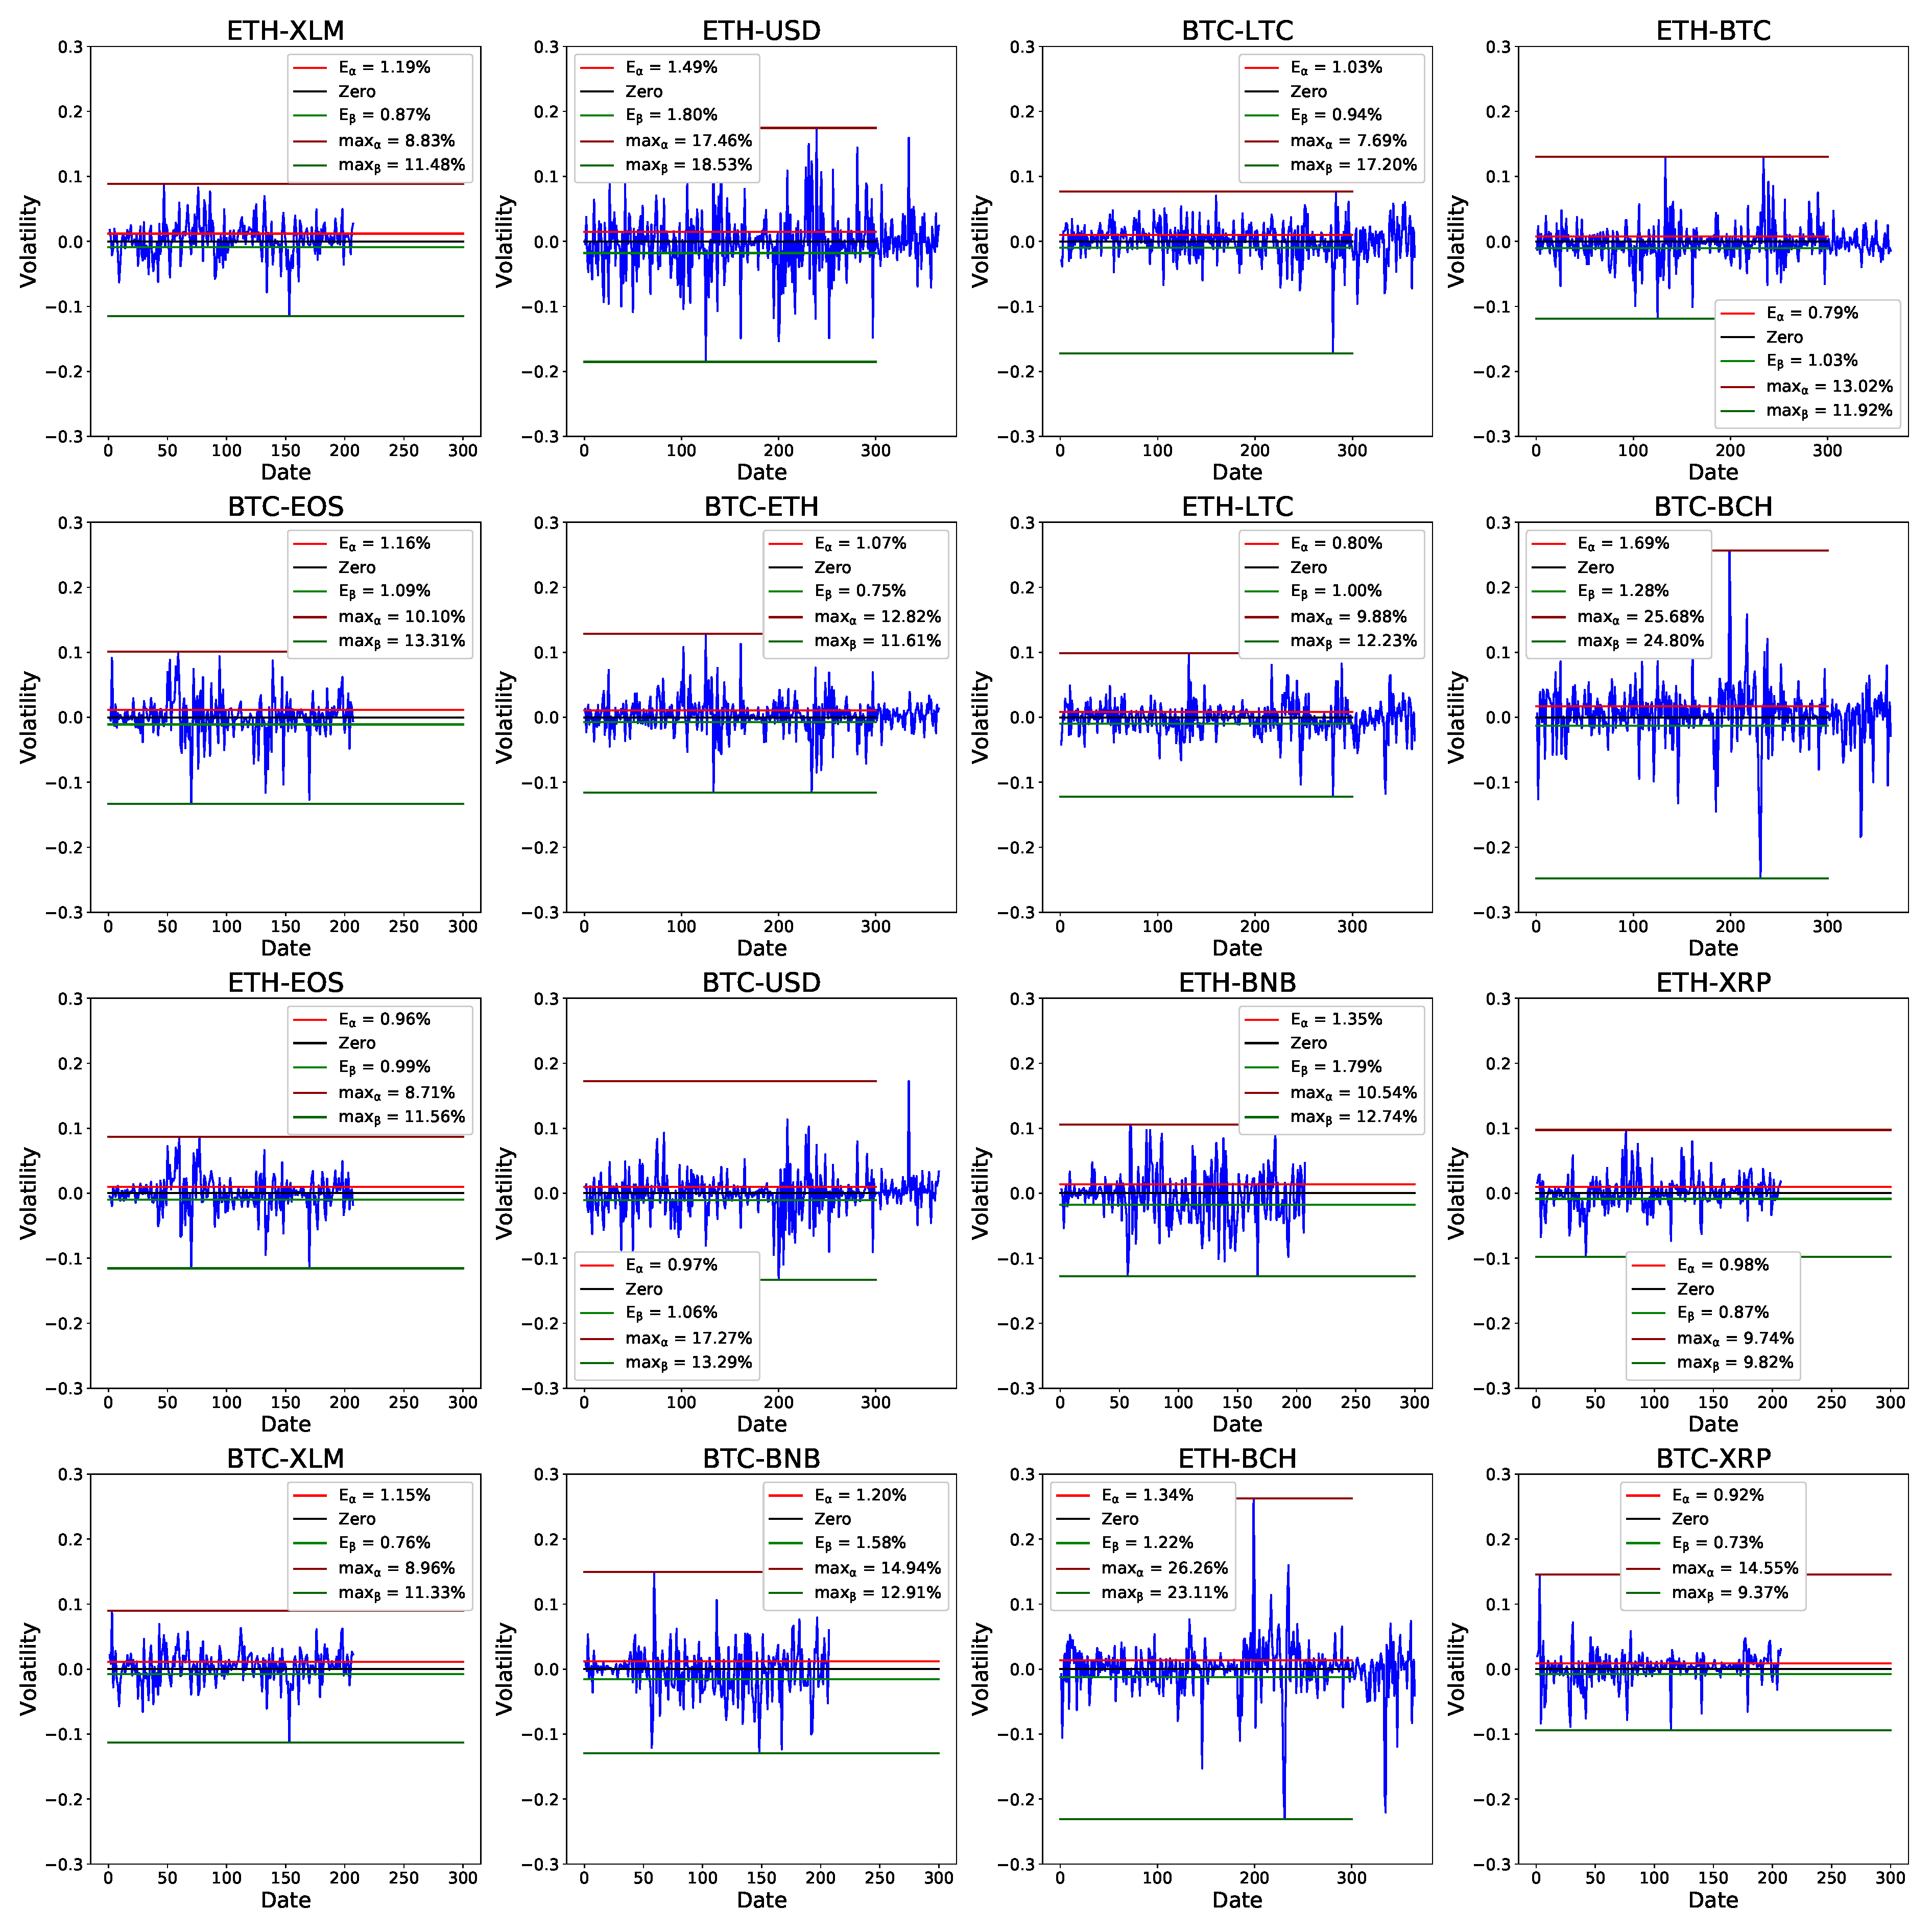
\includegraphics[width=\linewidth]{volatility_analysis.eps}
    \caption{The daily percentage changes for all selected cryptocurrency pairs, stock indices and fiat currency pairs over one year (from 03/05/2018 to 03/05/2019). For each figure, $E_{\alpha}$, $E_{\beta}$, $max_\alpha$ and $max_\beta$ are the expected profit rate, the expected mitigated risk rate, the maximum daily profit and the maximum daily mitigated risk, respectively.}
    \label{fig:volatility_analysis}
\end{figure*}

\begin{figure}
    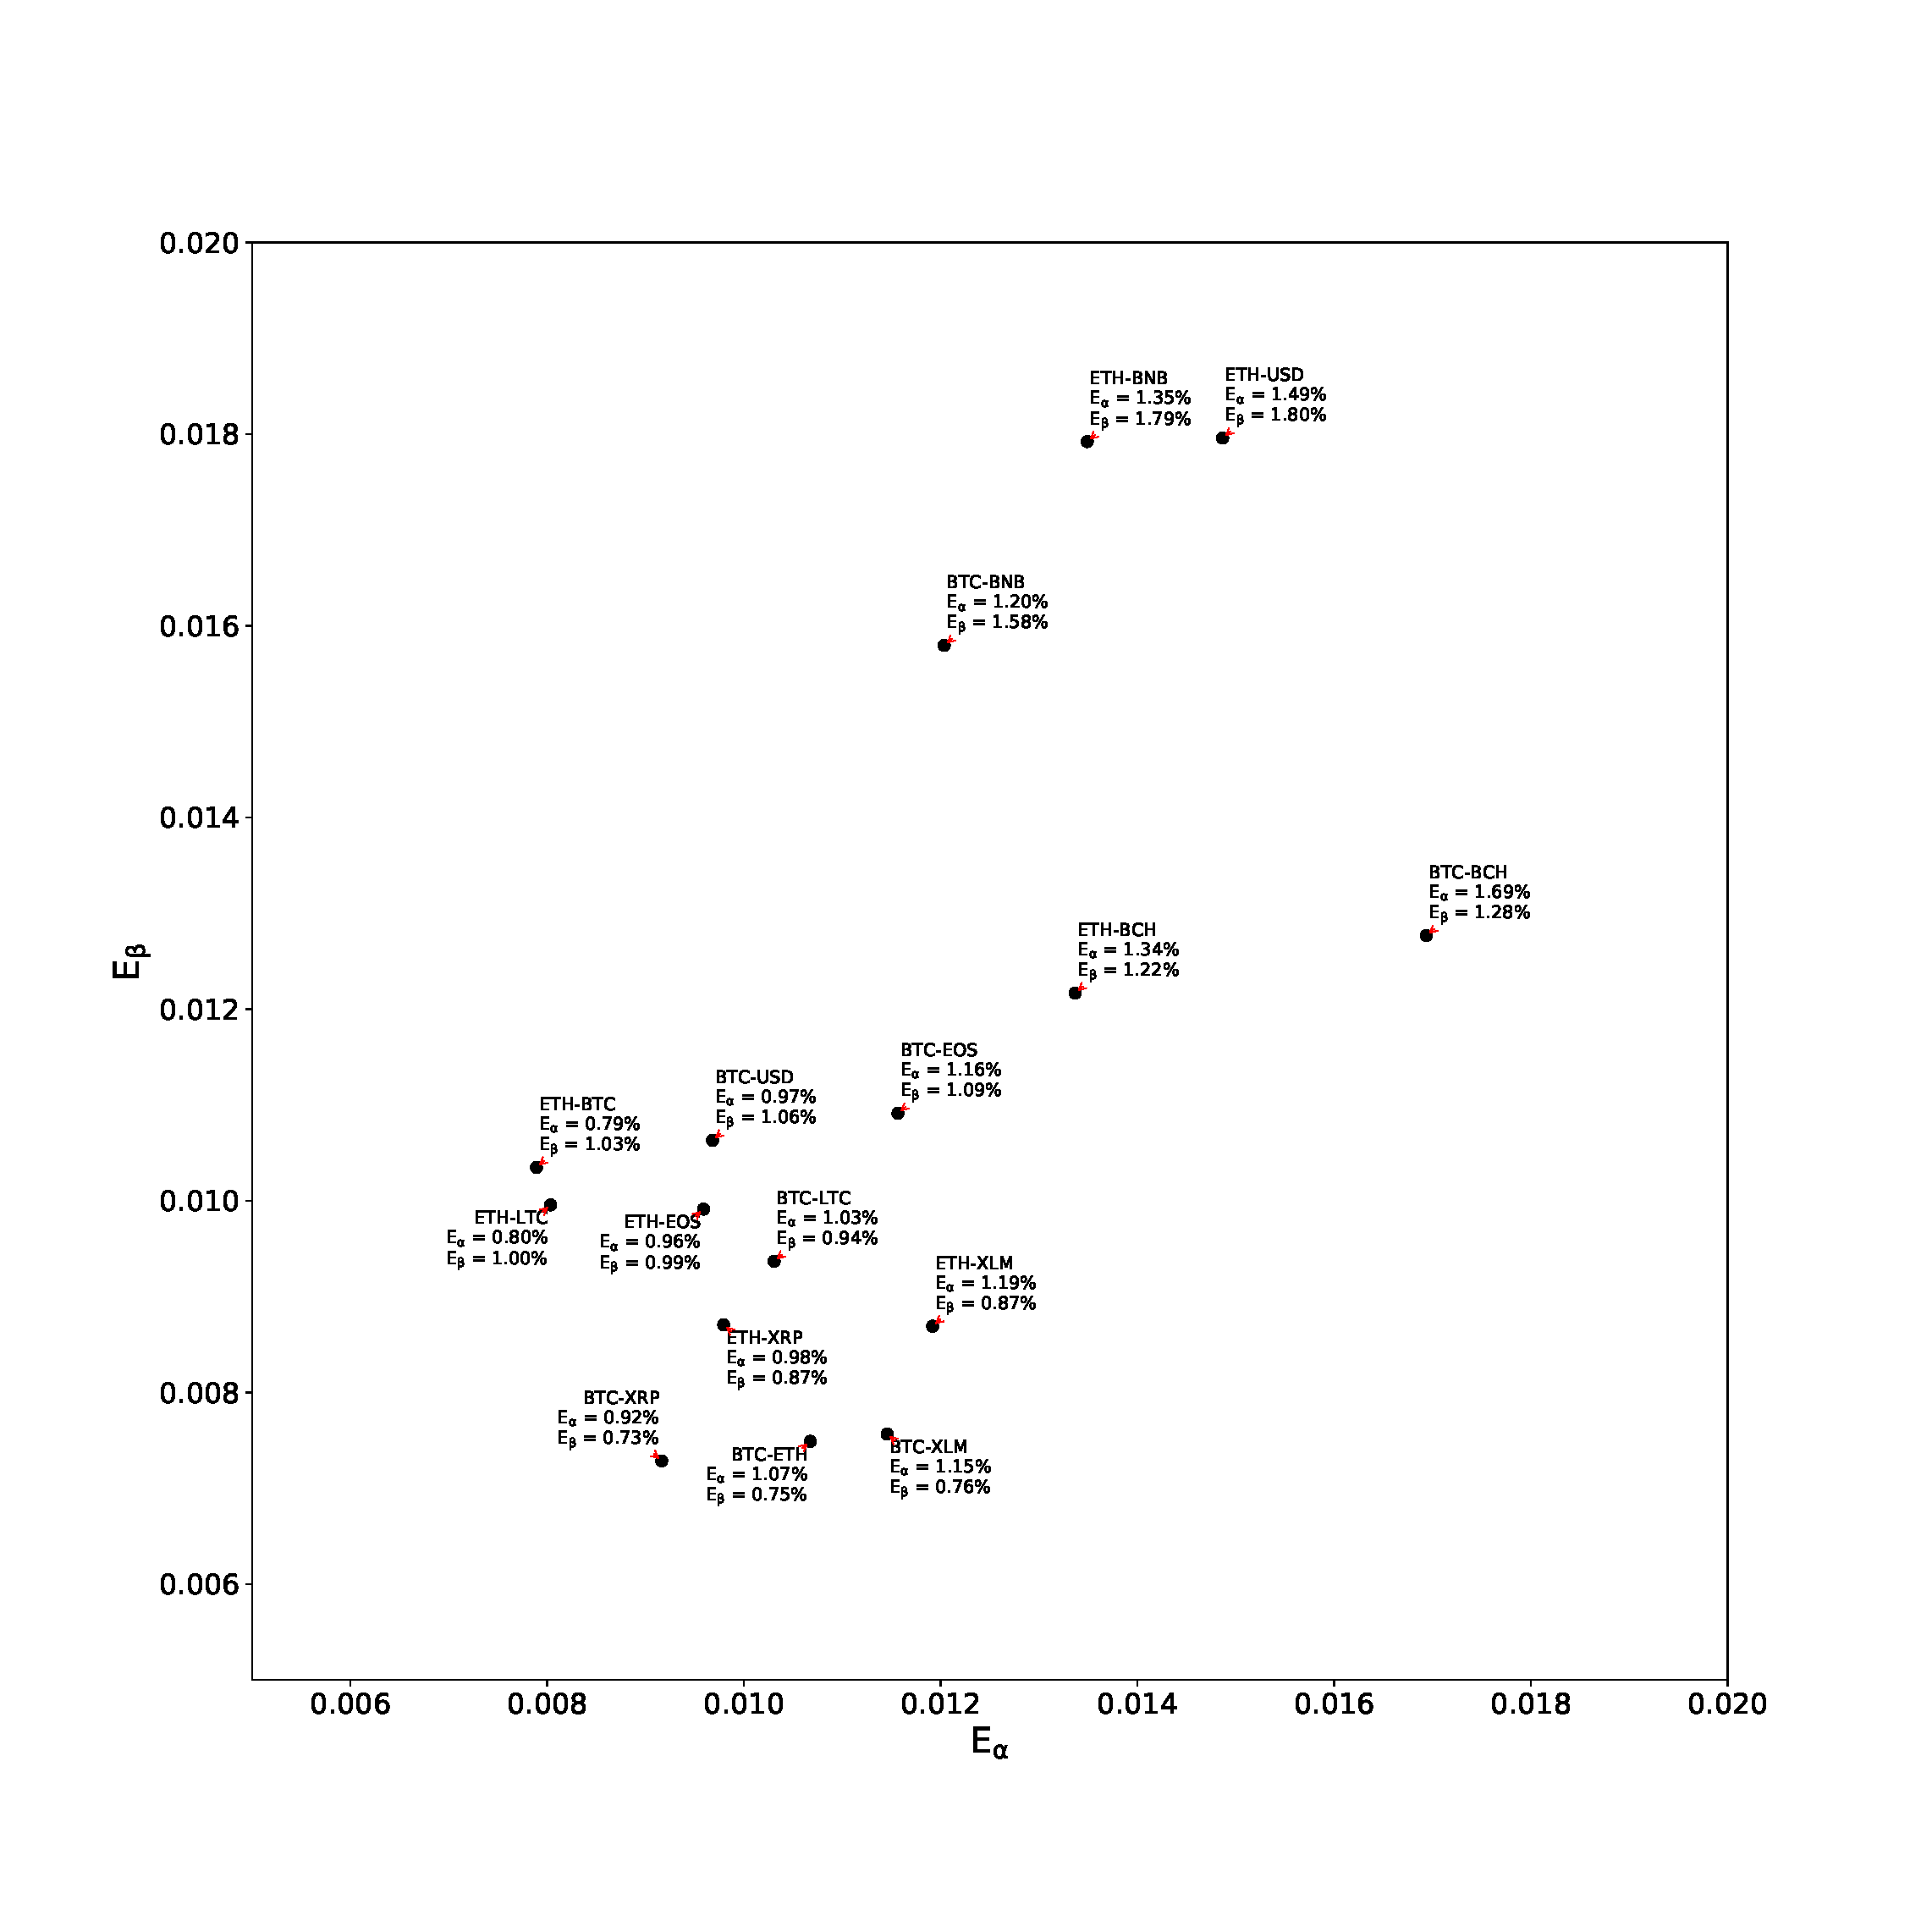
\includegraphics[width=\linewidth]{vol_scatter.eps}
    \caption{Visualizing the expected profit rate $E_\alpha$ and the expected mitigated risk rate $E_\beta$ for each cryptocurrency pair, stock index and fiat currency pair.}
    \label{fig:vol_scatter}
\end{figure}

Figure~\ref{fig:volatility_analysis} shows the estimated $E_\alpha$, $E_\beta$, the maximum daily rises $max_\alpha$ and the maximum \TODO{use \url{https://marketplace.visualstudio.com/items?itemName=ban.spellright} or \url{https://marketplace.visualstudio.com/items?itemName=streetsidesoftware.code-spell-checker} to avoid introducing typos?} daily drops $max_\beta$ for chosen 8 cryptocurrency pairs, stock indices (S\&P500 and DJI) and fiat currency exchange rates (USD-EUR and USD-GBP).
Figure~\ref{fig:vol_scatter} visualizes $E_\alpha$ and $E_\beta$ of all evaluated items in Figure~\ref{fig:volatility_analysis}.

\TODO{analysis may be improved}
We observe that for all chosen cryptocurrency pairs, $max_\alpha$ and $max_\beta$ are quite big - ranging from 8\% to 25\%.
Meanwhile, $max_\alpha$ and $max_\beta$ of stock indices are much smaller than all cryptocurrency pairs,
and $max_\alpha$ and $max_\beta$ of fiat currencies are even smaller than stock indices.
This indicates that in the setting of an 24-hour Atomic Swap, the cryptocurrency is much more unfair than stocks, and the stocks are more unfair than fiat currencies.

Also, for all chosen cryptocurrency pairs, $E_{\alpha}$ and $E_{\beta}$ are near and the value is approximately 1\%, ranging from 0.73\% to 1.69\%.
For stock indices, the results of S\&P500 and DJI are the same - $E_\alpha = 0.33\%$ and $E_\beta = 0.29\%$, which are smaller than cryptocurrency pairs.
For fiat currencies, $E_\alpha$ and $E_\beta$ are even smaller than stock indices: The value ranges from 0.13\% to 0.17\%.
In addition to the unfairness results like the previous observation, we quantify the unfairness of Atomic Swaps for cryptocurrency pairs: It ranges from  1.65\% (BTC-XRP) to 2.97\% (BTC-BCH).



















\subsection{Estimating the premium}

\MOD{The unfairness of the Atomic Swap comes from the fact that the initiator can abort the contract without punishment.
In Finance, the premium mechanism guarantees the good behaviours, which also works for Atomic Swaps.
Therefore, we can evaluate the unfairness of the Atomic Swap by estimating the premium for American Call Options with cryptocurrencies.}

As the premium is the only variable in an option contract, estimating the premium is also called the ``Option Pricing'' problem.
In finance, the Black-Scholes (BS) Model is utilized to price the European Call Options,
while the Cox-Ross-Rubinstein (CRR) Model is utilized to price the American Call Options.

Therefore, in order to evaluate the unfairness of the Atomic Swap, we utilize the CRR Model to estimate the premium for American Call Options with cryptocurrencies.

\subsubsection{The Cox-Ross-Rubinstein Model Explained}

The Cox-Ross-Rubinstein (CRR) Model~\cite{cox1979option} - a.k.a. the Binomial Options Pricing Model (BOPM) - provides a generalizable numerical method for pricing the options.
Intuitively, the CRR model enumerates all possible prices of the asset in the near future based on the price volatility,
then reverse-engineers the premium based on the enumerated prices.
% binomial tree
The model assume that for each step on the binomial tree, the asset price rises or falls by a fixed rate.
Enumerating the possible asset prices constructs a binomial tree, where each node attaches an asset price and a premium price at a point of time.
% reverse engineering
By iteratively back propagating the premium from the leaves to the root of the binomial tree, the premium will be revealed.

Formally, using the CRR model to price the American Call Option $\Pi = (\pi_1, \pi_2, K, A, T, C)$ with the underlying price $S_t$ of $\pi_2$ follows the steps below:
\begin{enumerate}
    \item Creating the binomial price tree
    \item Calculating the premiums for leaf nodes
    \item Iteratively reconstructing the premiums for non-leaf nodes 
\end{enumerate}


\begin{figure}
    \centering
    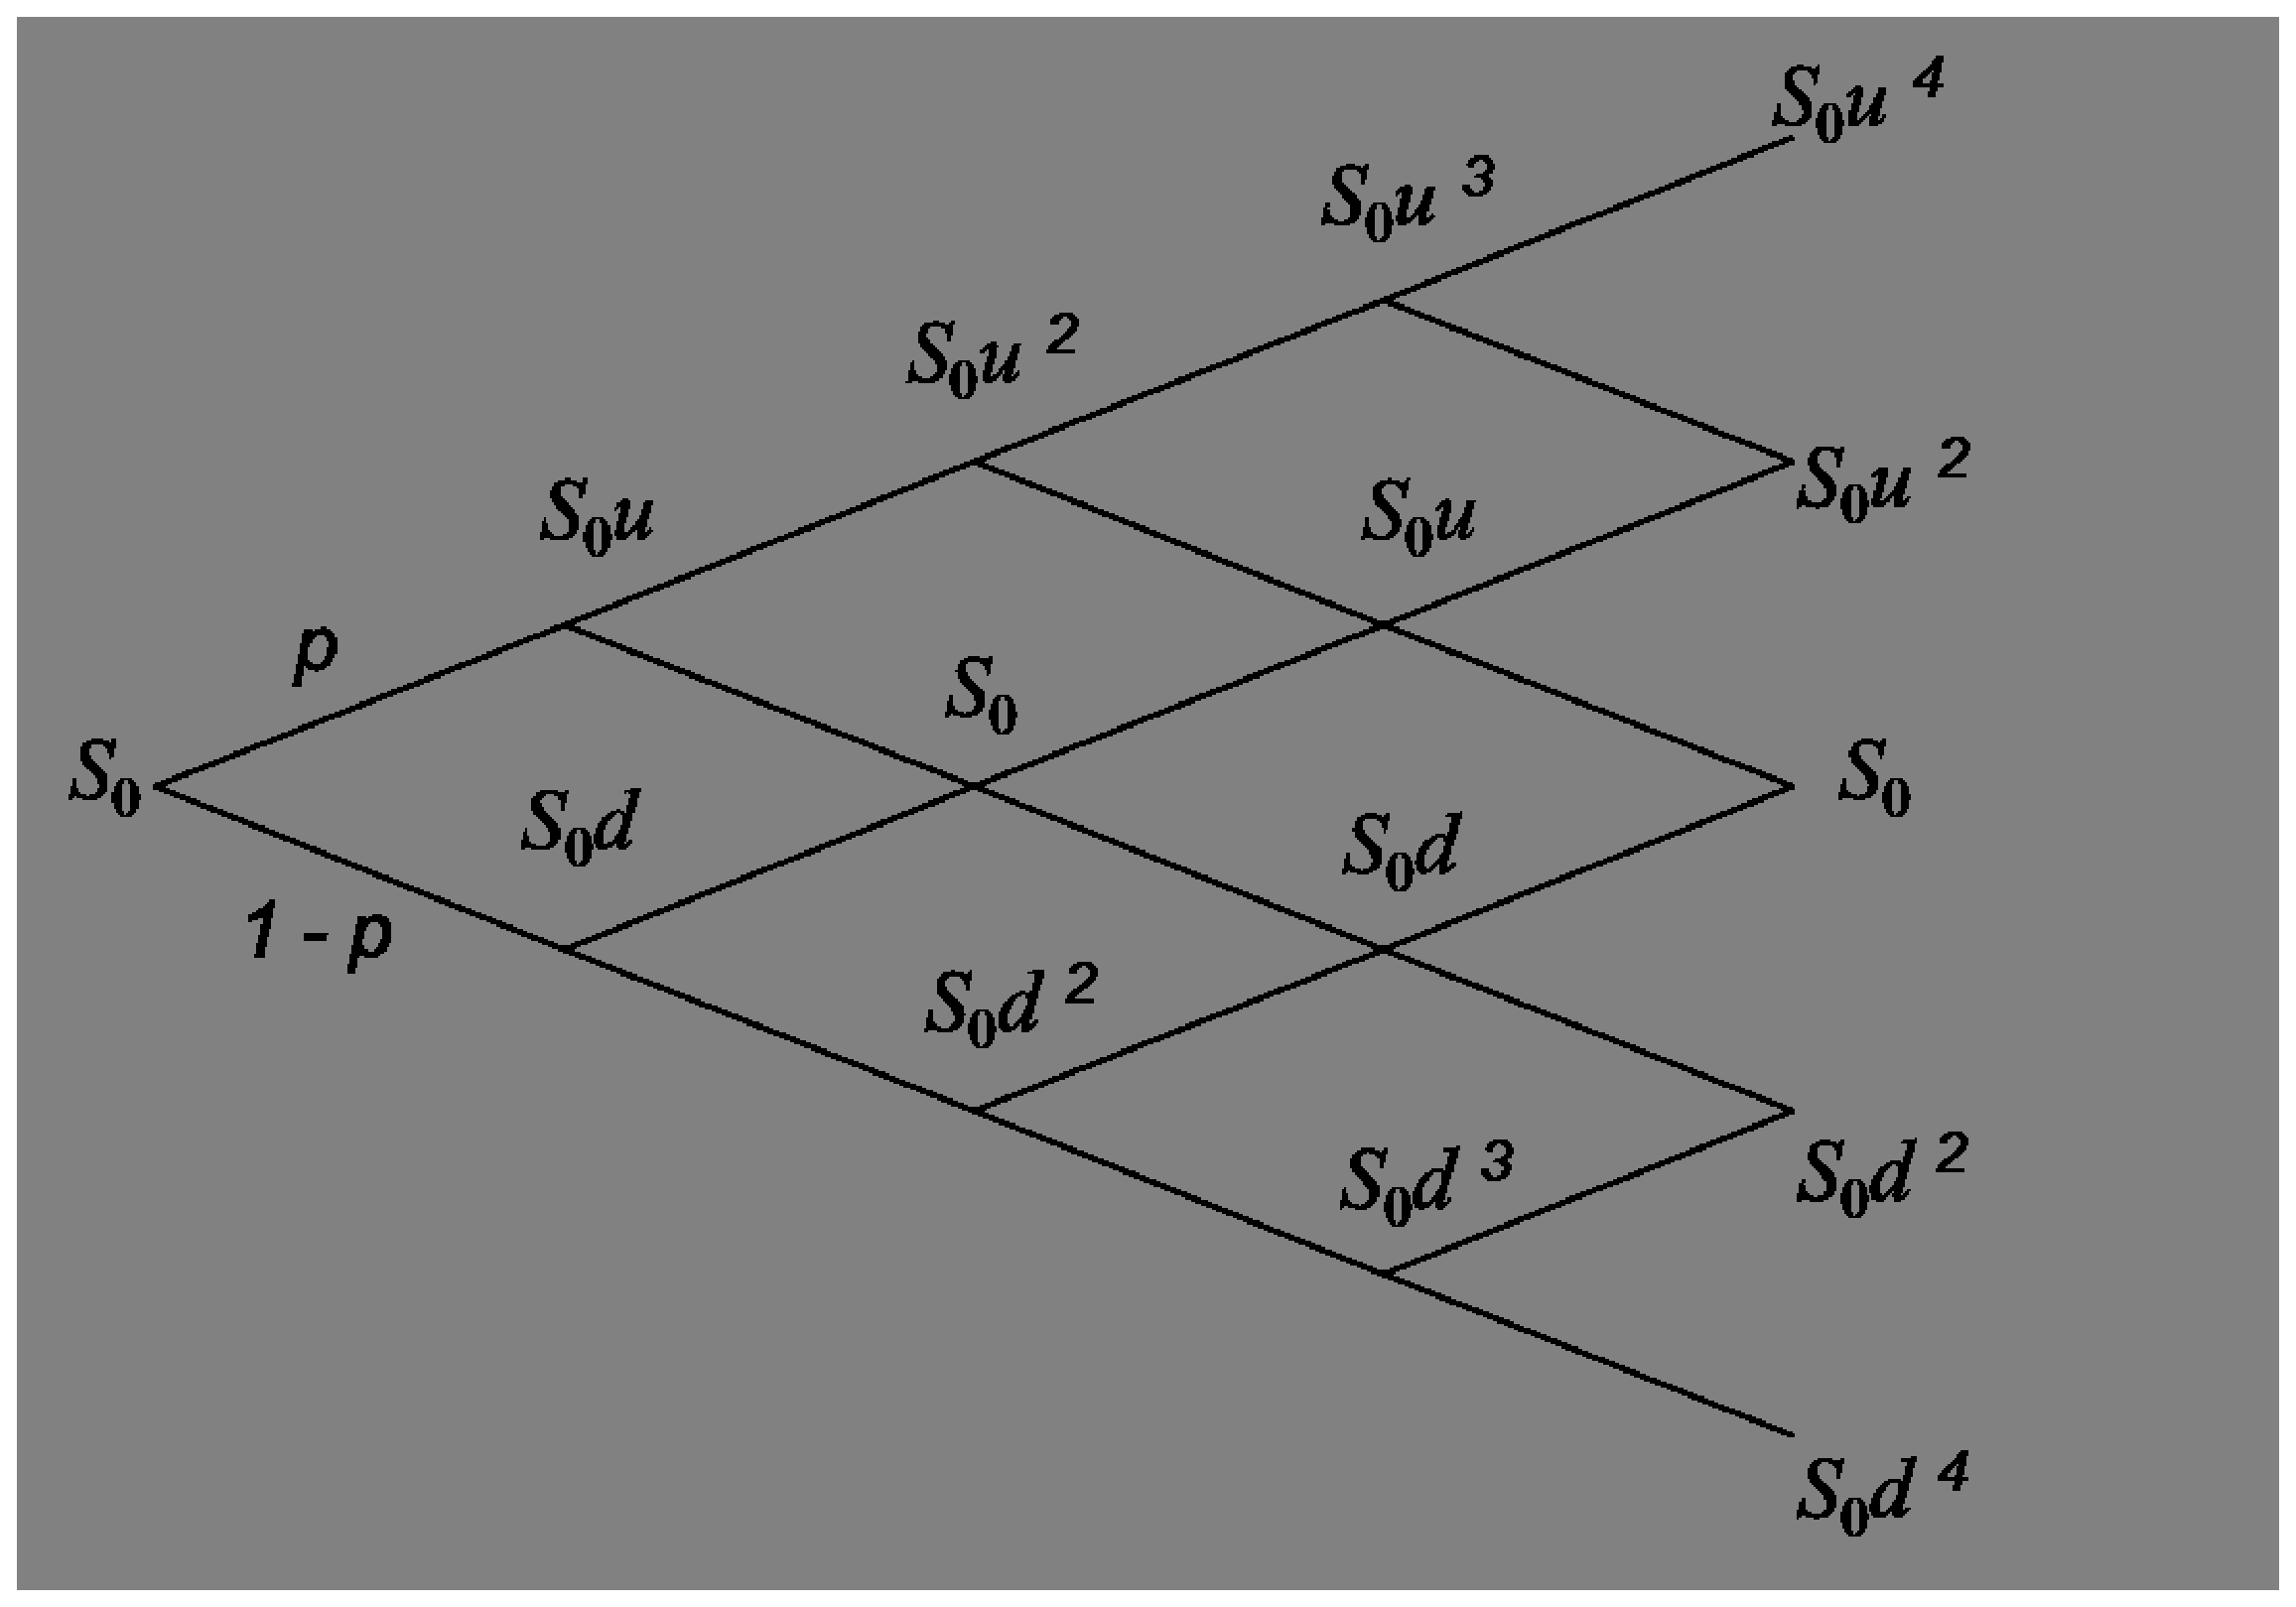
\includegraphics[width=\linewidth]{binomial-tree.eps}
    \caption{The binomial price tree $\mathcal{T}$. \JS{Maybe try to do it with tikz? This is a bit blurry atm. (added by Runchao)}}
    \label{fig:binomial_tree}
\end{figure}

\paragraph{Creating the binomial price tree.}
The binomial price tree $\mathcal{T}$ of the height $n$ represents the possible future prices within the time period $T$ discretely, as shown in Fig.~\ref{fig:binomial_tree}.
$n$ can be picked arbitrarily. With larger $n$, the result will be more accurate, but the computing overhead will be heavier.
Each node $\mathcal{T}_{t, i}$ is attached with the asset price $S_{t, i}$ and the premium $C_{t, i}$,
where $t \in \{0, \frac{T}{n}, \frac{2T}{n}, \dots, T\}$ is the point of time and $i$ is the number of the node at its level.
The CRR model assumes that the asset price will either move up or down by a specific factor per step in $\mathcal{T}$.
The move-up factor is $u$, and the move-down factor is $d$.
Accordingly, the price after one move-up is $S_{up} = u \cdot S$, and the price after one move-down is $S_{down} = d \cdot S$.
\JS{S is not defined. Is it possible to stay with the existing notation, i.e. $S_{t,i}$? (added by Runchao)}

$u$ and $d$ are calculated using the underlying annualized volatility $\sigma_a$ of the asset price:
\JS{It’s quite interesting, this seems to suggest that the drop and gain are symmetric, as $u\cdot d =1$. For example, if there is a high risk, then there will be high gain. (added by Runchao)}

\begin{align} 
u &= e^{\sigma_a \sqrt{\frac{T}{n}}}\\
d &= e^{- \sigma_a \sqrt{\frac{T}{n}}} = \frac{1}{u}
\end{align}

Here, $T$ is measured in years, and $\sigma_a$ is defined as the standard deviation of the annual price.
$\sigma_a$ can be computed from the daily price standard deviation $\sigma_d$ as below:

\begin{align} 
\sigma_a &= \sigma_d \sqrt{d}\\
\sigma_d &= \sqrt{\frac{\sum^{d}_{i=1} (S_i - \bar{S})^2}{d-1}}
\end{align}

where $d$ is the number of trading days within a year.
For cryptocurrencies, $d$ equals to the number of a days within a year.
Note that $S_i$ is the percentage change of the price on day $i$, rather than the price itself.
$\bar{S}$ is the average value of all $S_i$s within the $d$ days. 

The asset price $S_{t, i}$ can also be computed as $S_{t, i} = S_{0, 1} \cdot u^{N_u - N_d}$, where $S_{0, 1}$ is the spot price, and $N_u, N_d$ are the numbers of move-up and move-down, respectively.

\paragraph{Calculating the premiums for leaf nodes.}
In the first step, only the asset prices are determined rather than the premiums.
This step further determines the premiums for leaf nodes.
For each leaf node $\mathcal{T}_{n, i}$, the premium (for Call Options) is $C_{n, i} = max[(S_{n, i} - K), 0]$.

\paragraph{Iteratively reconstructing the premiums for earlier nodes.}
We back-propagate the premiums for leaf nodes to earlier premiums.
More specifically, the earlier premium is calculated from the premiums of the later two nodes weighted by their state transition possibilities.
The move-up and move-down possibility are $p$ and $q$ where $p + q = 1$, and the risk-free rate is $r = q$.

The earlier premium $C_{t - \Delta t, i}$ is calculated from later premiums as:

\begin{align}
C_{t - \Delta t, i} = e^{-r \Delta t} (p C_{t, i} + q C_{t, i+1})
\end{align}

where $\Delta t = \frac{T}{n}$, and $p, q, r$ are computed as

\begin{align} 
p &= \frac{e^{(r-q)\Delta t} - d}{u - d}\\
q &= 1 - p\\
r &= q
\end{align}

such that the premium distribution simulates the geometric Brownian motion with parameters $r$ and $\sigma$.

The earliest premium $S_{0, 1}$ - the estimated premium - can be calculated by iteratively back-propagating the later premiums. 

\JS{A table summarizing the notations will be nice — there are too many different notations, and I cannot remember them all. (added by Runchao)}

\subsubsection{Experiments}


\begin{figure}
    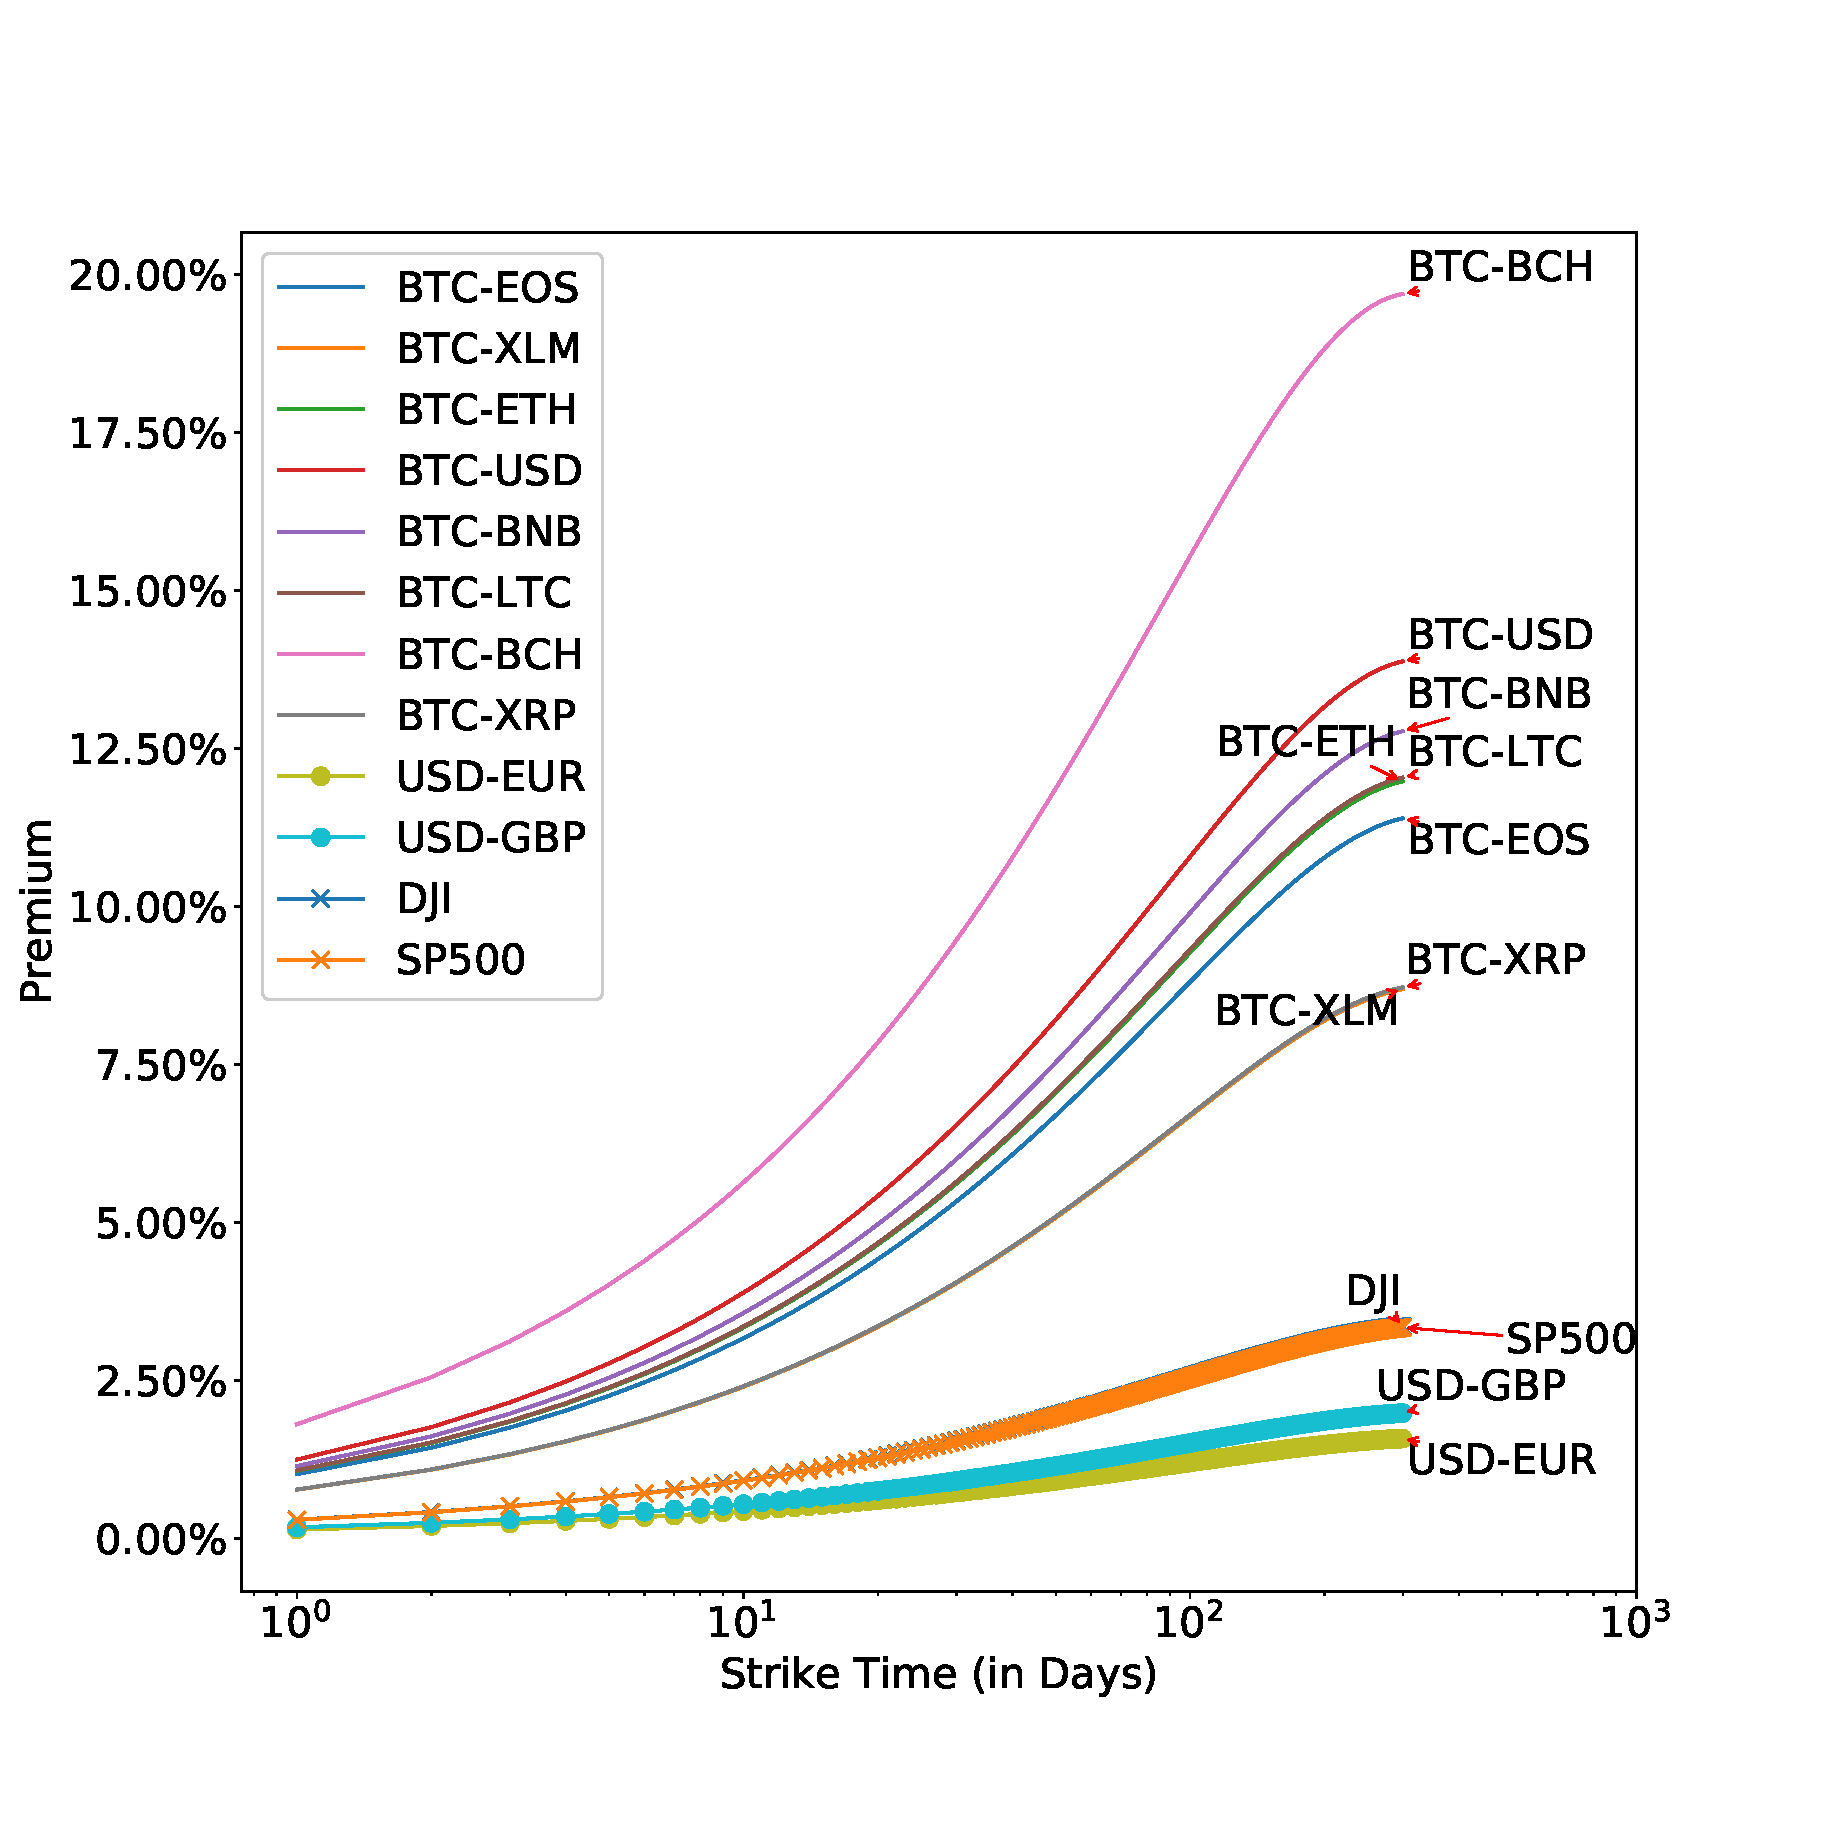
\includegraphics[width=\linewidth]{premium_pricing_result.eps}
    \caption{Estimated premium with different strike times for each cryptocurrency pair, stock index and fiat currency pair. Lines with the marker ``x'' are for stocks; lines with the marker ``o'' are for fiat currencies; and lines without marker are for cryptocurrency pairs.}
    \label{fig:premium_pricing_result}
\end{figure}

We price the same data as Section~\ref{subsec:volatility_analysis} by using the CRR model with $n = 36$ with the strike time $T$ ranging from $1$ to $300$.
Figure~\ref{fig:premium_pricing_result} shows our pricing results.

First, we observe that the premium of cryptocurrency pairs is much more expensive than stocks, and the premium of stocks is more expensive than fiat currencies at any given time.
Recall the evaluated unfairness in Section~\ref{subsec:volatility_analysis}, its results are consistent with the premium pricing results: The higher the volatility is, the more unfair the Atomic Swap will be, and the higher the premium should be.

Second, with the default strike time $T = 1$ of the Atomic Swap, the premium of cryptocurrency pairs vary from approximately 1\% to 2.3\% of the underlying asset value.

Third, for all evaluated items, the premium values rise monotonically.
This is because the longer expiration time lets the option buyer to have more control on the option - He has more time to predict the price and judges whether to exercise the option.
\section{Fair Atomic Swaps: Marketizing the Premium}
\label{sec:fairer_atomic_swap}

\subsection{Design Rationale}

The CRR model estimates how much the premium should be, rather than how much the premium is exactly.
In reality, the premium is marketized by investors, and regulated by the government.

\subsection{Our Construction}
\section{Implementation}
\label{sec:implementation}

In this section, we describe how to implement our proposed protocols in Section~\ref{sec:fair_atomic_swap} on different blockchains, including blockchains only supporting scripts (such as Bitcoin) and blockchains supporting smart contracts (such as Ethereum).
In particular, we describe our design rationale, and provide reference implementations in Bitcoin scripts and Solidity smart contracts.

\subsection{Requirements}

To implement our protocols, the blockchain should support the following functionalities:

\begin{enumerate}
    \item Stateful transactions
    \item Timelock
    \item Hashlock
\end{enumerate}

\paragraph{Stateful transactions}
Transactions should be stateful: Executing a transaction can depend on prior transactions.
In our protocols, whether $pr$ goes to Alice or Bob depends on the status of $Coin_2$.
Therefore, the transaction of $pr$ relies on the status of $Coin_2$ payment transaction.

\paragraph{Hashlock}
The transactions should support the hashlock: A payment is proceeded only when the payee provides the preimage of a hash.
In our protocols, exchanging $Coin_1$ and $Coin_2$ atomically is based on the hashlock -
Alice redeems $Coin_2$ first by releasing the preimage, then Bob can redeem $Coin_1$ by using the released preimage.

\paragraph{Timelock}
The transactions should support the timelock: A payment will expire after a specified time if the payee cannot redeem the payment.
Note that the payment can be conditional, e.g. by hashlock.
In our protocols, the transactions of $Coin_1$, $Coin_2$ and $pr$ are all timelocked, in order to avoid locking money in transactions forever.

\subsection{Smart contracts}

Smart contracts support all aforementioned functionalities, so can easily implement our protocols.
We use the Solidity - the programming language for Ethereum smart contracts~\cite{wood2014ethereum} - as an example.

Our implementations are based on the original Atomic Swap Solidity implementation~\footnote{\url{https://github.com/AltCoinExchange/ethatomicswap}.},
but extend the premium mechanism.

Extending the premium mechanism includes:

\begin{enumerate}
    \item The enumeration \textit{AssetState} for maintaining the premium payment state
    \item The modifiers \textit{isPremiumRedeemable()} and \textit{isPremiumRefundable()} for checking whether the premium can be redeemed or refunded
    \item The methods \textit{redeemPremium()} and \textit{refundPremium()} for redeeming and refunding the premium
\end{enumerate}

\paragraph{The premium payment state \textit{AssetState}}

\begin{figure}[htb]
\begin{lstlisting}[
    language=Solidity, 
    basicstyle=\tiny,
    label={lst:state},
    caption={Maintaining the state of the asset and the premium.}
]
enum AssetState { Empty, Filled, Redeemed, Refunded }
enum PremiumState { Empty, Filled, Redeemed, Refunded }
\end{lstlisting}
\end{figure}

\begin{figure}[htb]
\begin{lstlisting}[
    language=Solidity, 
    basicstyle=\tiny,
    label={lst:premium_condition_currency},
    caption={The condition to redeem and refund the premium for currency-exchange-style Atomic Swaps.}
]
// Premium is refundable when
// 1. Alice initiates but Bob does not participate
//   after premium's timelock expires
// 2. asset2 is redeemed by Alice
modifier isPremiumRefundable(bytes32 secretHash) {
    // the premium should be deposited
    require(swaps[secretHash].premiumState == PremiumState.Filled);
    // the initiator invokes this method to refund the premium
    require(swaps[secretHash].initiator == msg.sender);
    // the contract should be on the blockchain2
    require(swaps[secretHash].kind == Kind.Participant);
    // if the asset2 timelock is still valid
    if block.timestamp <= swaps[secretHash].assetRefundTimestamp {
        // the asset2 should be redeemded by Alice
        require(swaps[secretHash].assetState == AssetState.Redeemed);
    } else { // if the asset2 timelock is still valid
        // the asset2 should not be refunded
        require(swaps[secretHash].assetState != AssetState.Refunded);
        // the premium timelock should be expired
        require(block.timestamp > swaps[secretHash].premiumRefundTimestamp);
    }
    _;
}
// Premium is redeemable for Bob when asset2 is refunded
// which means Alice holds the secret maliciously
modifier isPremiumRedeemable(bytes32 secretHash) {
    // the premium should be deposited
    require(swaps[secretHash].premiumState == PremiumState.Filled);
    // the participant invokes this method to redeem the premium
    require(swaps[secretHash].participant == msg.sender);
    // the contract should be on the blockchain2
    require(swaps[secretHash].kind == Kind.Participant);
    // the asset2 should be refunded
    // this also indicates the asset2 timelock is expired
    require(swaps[secretHash].assetState == AssetState.Refunded);
    // the premium timelock should not be expired
    require(block.timestamp <= swaps[secretHash].premiumRefundTimestamp);
    _;
}
\end{lstlisting}
\end{figure}

\begin{figure}[htb]
\begin{lstlisting}[
    language=Solidity, 
    basicstyle=\tiny,
    label={lst:premium_condition_options},
    caption={The condition to redeem and refund the premium for American Call Option-style Atomic Swaps.}
]
// Premium is refundable for Alice only when Alice initiates
// but Bob does not participate after premium's timelock expires
modifier isPremiumRefundable(bytes32 secretHash) {
    // the premium should be deposited
    require(swaps[secretHash].premiumState == PremiumState.Filled);
    // the initiator invokes this method to refund the premium
    require(swaps[secretHash].initiator == msg.sender);
    // the contract should be on the blockchain2
    require(swaps[secretHash].kind == Kind.Participant);
    // premium timelock should be expired
    require(block.timestamp > swaps[secretHash].premiumRefundTimestamp);
    // asset2 should be empty
    // which means Bob does not participate
    require(swaps[secretHash].assetState == AssetState.Empty);
}
// Premium is redeemable for Bob when asset2 is redeemed or refunded
// which means Bob participates
modifier isPremiumRedeemable(bytes32 secretHash) {
    // the premium should be deposited
    require(swaps[secretHash].premiumState == PremiumState.Filled);
    // the participant invokes this method to redeem the premium
    require(swaps[secretHash].participant == msg.sender);
    // the contract should be on the blockchain2
    require(swaps[secretHash].kind == Kind.Participant);
    // the asset2 should be refunded or redeemed
    require(swaps[secretHash].assetState == AssetState.Refunded || swaps[secretHash].assetState == AssetState.Redeemed);
    // the premium timelock should not be expired
    require(block.timestamp <= swaps[secretHash].premiumRefundTimestamp);
    _;
}
\end{lstlisting}
\end{figure}

Similar with the \textit{PremiumState}, \textit{AssetState} has 4 states: empty, filled, redeemded and refunded.
The code is shown in Listing~\ref{lst:state}.
\textit{Empty} means Alice has not \textbf{initiate}d, and has not deposited the premium yet.
\textit{Filled} means Alice has deposited the premium, indicating that Alice has \textbf{initiate}d, but neither Alice nor Bob \textbf{refund}s or \textbf{redeem}s the premium.
\textit{Redeemded} and \textit{refunded} means Bob redeems the premium and Alice refunds the premium, respectively.

\paragraph{\textit{isPremiumRedeemable()} and \textit{isPremiumRefundable()}}
Checking whether the premium is redeemable or refundable is the most critical part of our protocols.
Because the premium payment relies on the $Coin_2$ payment, checking the premium refundability and redeemability involves checking the $Coin_2$ status - \textit{AssetState} in our implementation.

\textit{isPremiumRedeemable()} and \textit{isPremiumRefundable()} for the currency exchange-style Atomic Swap are shown in Figure~\ref{lst:premium_condition_currency}, and for the American Call Option-style Atomic Swap are shown in Figure~\ref{lst:premium_condition_options}.
The currency exchange-style Atomic Swap and the American Call Option-style Atomic Swap differ when $AssetState = Redeemed$:
In the currency exchange-style Atomic Swap the premium belongs to Alice while in the American Call Option-style Atomic Swap the premium belongs to Bob.

\paragraph{\textit{redeemPremium()} and \textit{refundPremium()}}

\textit{redeemPremium()} and \textit{refundPremium()} are similar with \textit{redeemAsset()} and \textit{refundAsset()}, and their executions are secured by \textit{isPremiumRedeemable()} and \textit{isPremiumRefundable()}.
The code is shown in Listing~\ref{lst:premium_redeem_refund_function}.

\begin{figure}[htb]
\begin{lstlisting}[
    language=Solidity, 
    basicstyle=\tiny,
    label={lst:premium_redeem_refund_function},
    caption={The functions for redeeming and refunding the premium.}
]
function redeemPremium(bytes32 secretHash)
    public
    isPremiumRedeemable(secretHash)
{
    // transfer the premium to Bob
    swaps[secretHash].participant.transfer(swaps[secretHash].premiumValue);
    // update the premium state to redeemded
    swaps[secretHash].premiumState = PremiumState.Redeemed;
    // notify the function invoker
    emit PremiumRefunded(
        block.timestamp,
        swaps[secretHash].secretHash,
        msg.sender,
        swaps[secretHash].premiumValue
    );
}
    function refundPremium(bytes32 secretHash)
    public
    isPremiumRefundable(secretHash)
{
    // transfer the premium to Alice
    swaps[secretHash].initiator.transfer(swaps[secretHash].premiumValue);
    // update the premium state to refunded
    swaps[secretHash].premiumState = PremiumState.Refunded;
    // notify the function invoker
    emit PremiumRefunded(
        block.timestamp,
        swaps[secretHash].secretHash,
        msg.sender,
        swaps[secretHash].premiumValue
    );
}
\end{lstlisting}
\end{figure}

\subsection{Bitcoin script}

% bitcoin cannot implement
% because stateless
Unfortunately, Bitcoin does not support our protocols, because Bitcoin does not support the stateful transaction functionalities.
First, the Bitcoin script is designed to be stateless~\cite{okupski2014bitcoin}.
Second, there is no such things like the Ethereum's ``world state''~\cite{wood2014ethereum} in Bitcoin:
The only state in Bitcoin is the Unspent Transaction Outputs (UTXOs)~\cite{nakamoto2008bitcoin}.


% new opcode
\paragraph{New Opcode OP\_LOOKUP\_OUTPUT}
In order to make Bitcoin script support our protocols, we use an opcode called OP\_LOOKUP\_OUTPUT.
OP\_LOOKUP\_OUTPUT was proposed, but has not implemented in Bitcoin yet~\cite{op-lookup-output-origin}.
It takes the id of an output, and produces the address of the output's owner.
With OP\_LOOKUP\_OUTPUT, the Bitcoin script can decide whether Alice or Bob should take the premium by
``<asset2\_output> OP\_LOOKUP\_OUTPUT <Alice\_pubkeyhash> OP\_EQUALVERIFY''.

% implement opcode is easy
Implementing OP\_LOOKUP\_OUTPUT is easy in Bitcoin - It only queries the ownership of an output from the indexed blockchain database.
This neither requires any computation, nor breaks the ``stateless'' design of the Bitcoin script.


\paragraph{Decoupling the contract creation and the contract invocation}
For smart contracts, the contract is created and invoked in separate transactions:
Creating the contract is by publishing a transaction which creates the smart contract,
and invoking the contract is by publishing a transaction which invokes a method in the smart contract.
However, Bitcoin has no smart contracts, and the ``contract'' is created and invoked in a single transaction.
In this way, the timelock starts right after the contract creation rather than the contract invocation.
This is problematic: The contract is invoked when Bob \textbf{participate}s in the contract.


Thanks to the multi-signature transaction functionality in Bitcoin,
Alice and Bob can first create the contract off-chain, then invoke the contract on-chain.

Multi-signature transactions refer to transactions signed by multiple accounts~\cite{okupski2014bitcoin}.
A M-of-N ($M \leq N$) multi-signature transaction means the transaction requires $M$ out of $N$ accounts to sign it.
If less than $M$ accounts sign the transaction, the transaction cannot be verified as valid by blockchain participants.
In Bitcoin, constructing a multi-signature transaction requires accounts to create a multi-signature address first~\cite{okupski2014bitcoin}.

With multi-signature transactions, we can decouple the contract creation and invocation as follows:
First, Alice and Bob create a 2-of-2 multi-signature address. 
Second, Alice and Bob mutually construct and sign a transaction which includes the premium payment and the $Coin_2$ payment.
Finally, both Alice and Bob sign and publish the transaction with the 2-2 multi-signature address.

Note that the second step above is done off-chain:
First, Bob creates the $Coin_2$ transaction and sends it to Alice.
Second, Alice creates the premium transaction which uses OP\_LOOKUP\_OUTPUT to check the ownership of $Coin_2$ transaction outputs.
Third, Alice merges the $Coin_2$ transaction and the premium transaction to a single transaction, signs the transaction, and sends it to Bob.
Finally, Bob signs the transaction and sends it to Alice.
At this stage, both Alice and Bob have the mutually signed transaction containing both the premium transaction and the $Coin_2$ transaction.

\paragraph{The premium transaction}
Listing~\ref{lst:bitcoin_contract_currency_exchange} and Listing~\ref{lst:bitcoin_contract_option} show the premium transaction in the Bitcoin script
, for both the currency-style and the American Call Option-style Atomic Swaps, respectively.

\begin{figure}[htb]
\begin{lstlisting}[
    language=Solidity, 
    basicstyle=\tiny,
    label={lst:bitcoin_contract_currency_exchange},
    caption={The currency exchange-style Atomic Swap contract in Bitcoin script.}
]
ScriptSig:
    Redeem: <Bob_sig> <Bob_pubkey> 1
    Refund: <Alice_sig> <Alice_pubkey> 0
ScriptPubKey:
    OP_IF // Normal redeem path
        // the owner of <asset2_output> should be Alice
        // which means Alice has redeemed asset2
        <asset2_output> OP_LOOKUP_OUTPUT <Alice_pubkeyhash> OP_EQUALVERIFY 
        OP_DUP OP_HASH160 <Bob_pubkeyhash>
    OP_ELSE // Refund path
        // the premium timelock should be expired
        <locktime> OP_CHECKLOCKTIMEVERIFY OP_DROP
        OP_DUP OP_HASH160 <Alice pubkey hash>
    OP_ENDIF
    OP_EQUALVERIFY
    OP_CHECKSIG
\end{lstlisting}  
\end{figure}

\begin{figure}[htb]
\begin{lstlisting}[
    language=Solidity, 
    basicstyle=\tiny,
    label={lst:bitcoin_contract_option},
    caption={The American Call Option-style Atomic Swap contract in Bitcoin script.}
]
ScriptSig:
    Redeem: <Bob_sig> <Bob_pubkey> 1
    Refund: <Alice_sig> <Alice_pubkey> 0
ScriptPubKey:
    OP_IF // Normal redeem path
        // the owner of the asset2 should not be the contract
        // it should be either (redeemde by) Alice or (refunded by) Bob
        // which means Alice has redeemed asset2
        <asset2_output> OP_LOOKUP_OUTPUT <Alice_pubkeyhash> OP_NUMEQUAL
        <asset2_output> OP_LOOKUP_OUTPUT <Bob_pubkeyhash> OP_NUMEQUAL
        OP_ADD 1 OP_NUMEQUALVERIFY
        OP_DUP OP_HASH160 <Bob_pubkeyhash>
    OP_ELSE // Refund path
        // the premium timelock should be expired
        <locktime> OP_CHECKLOCKTIMEVERIFY OP_DROP
        OP_DUP OP_HASH160 <Alice pubkey hash>
    OP_ENDIF
    OP_EQUALVERIFY
    OP_CHECKSIG
\end{lstlisting}
\end{figure}

% OP_LOOKUP_OUTPUT is from https://bitcoin.stackexchange.com/questions/36229/bitcoin-script-for-a-competitive-crowdfunding-like-contract
\section{Discussion}
\label{sec:discussion}

\subsection{Other Countermeasures for Speculative Atomic Cross-Chain Swaps}

\subsection{Limitations}
\section{Related Work}
\label{sec:related_work}

\paragraph{Atomic Swaps}
The Atomic Swap protocol was first proposed on the BitcoinTalk forum informally in 2013~\cite{nolan2013alt}.
Herlihy et al. first formalised the Atomic Swap protocol~\cite{herlihy2018atomic}.
Meyden et al. first formally analysed the Atomic Swap smart contracts~\cite{van2018specification}.
Several Atomic Swap variants were proposed for sidechains~\cite{robinson2019atomic} and solving conflicts due to concurrent operations~\cite{zakhary2019atomic}.

\paragraph{Optionality of Atomic Swaps}
The optionality of Atomic Swaps was first identified by an anonymous person entitled ZmnSCPxj in the Lightning-dev mail list in 2018~\cite{optionality-origin}.
Eizinger et al. first tried to address the optionality problem by implementing the premium mechanism in the Atomic Swap\cite{first-attempt-optionality}.
Liu et al. used the Atomic Swap to construct the option~\cite{liu2018atomic}, but paying for the premium requires an extra blockchain besides the two blockchains, and they do not justify its fairness.

\paragraph{Option Pricing}
The Black-Scholes model is the first model to price the European options~\cite{black1973pricing}.
The Cox-Ross-Rubinstein extended the Black-Scholes to price the American Options~\cite{cox1979option}.
\section{Conclusion}
\label{sec:conclusion}


In this paper, we investigate the fairness of Atomic Swap.
We show that an Atomic Swap is equivalent to a premium-free American Call Option, and Atomic Swap is unfair to the participant.

% quantify
We then evaluate the fairness of Atomic Swap protocol, and compare the fairness between mainstream cryptocurrencies and conventional financial assets.
Our evaluation consists of quantifying the fairness and estimating the unpaid premium.
The evaluation results show that the Atomic Swap with cryptocurrencies is much more unfair than with stocks and fiat currencies in the same setting, because the cryptocurrency market is highly volatile.

% propose
Furthermore, we propose an improvement on Atomic Swap, which implements the premium mechanism, to make it fair.
It supports both the currency exchange-style Atomic Swap, and the American Call Option-style Atomic Swap.
We implement our protocol in Solidity as an example of blockchains with smart contracts such as Ethereum.
We also give instructions on implementing our protocol using Bitcoin script, which requires adding a single opcode to the Bitcoin script.

\begin{acks}
We thank Sungying Chen and Xin Lin for providing their knowledge on option pricing models in finance.
We thank ZmnSCPxj for the discussion on implementing our protocol on Bitcoin.
We also thank anonymous reviewers for their constructive feedback.
\end{acks}

\printbibliography

\newpage

\appendix

\section{Sequence diagrams}

\begin{figure*}[t]
\centering
    \begin{subfigure}{.3\textwidth}
        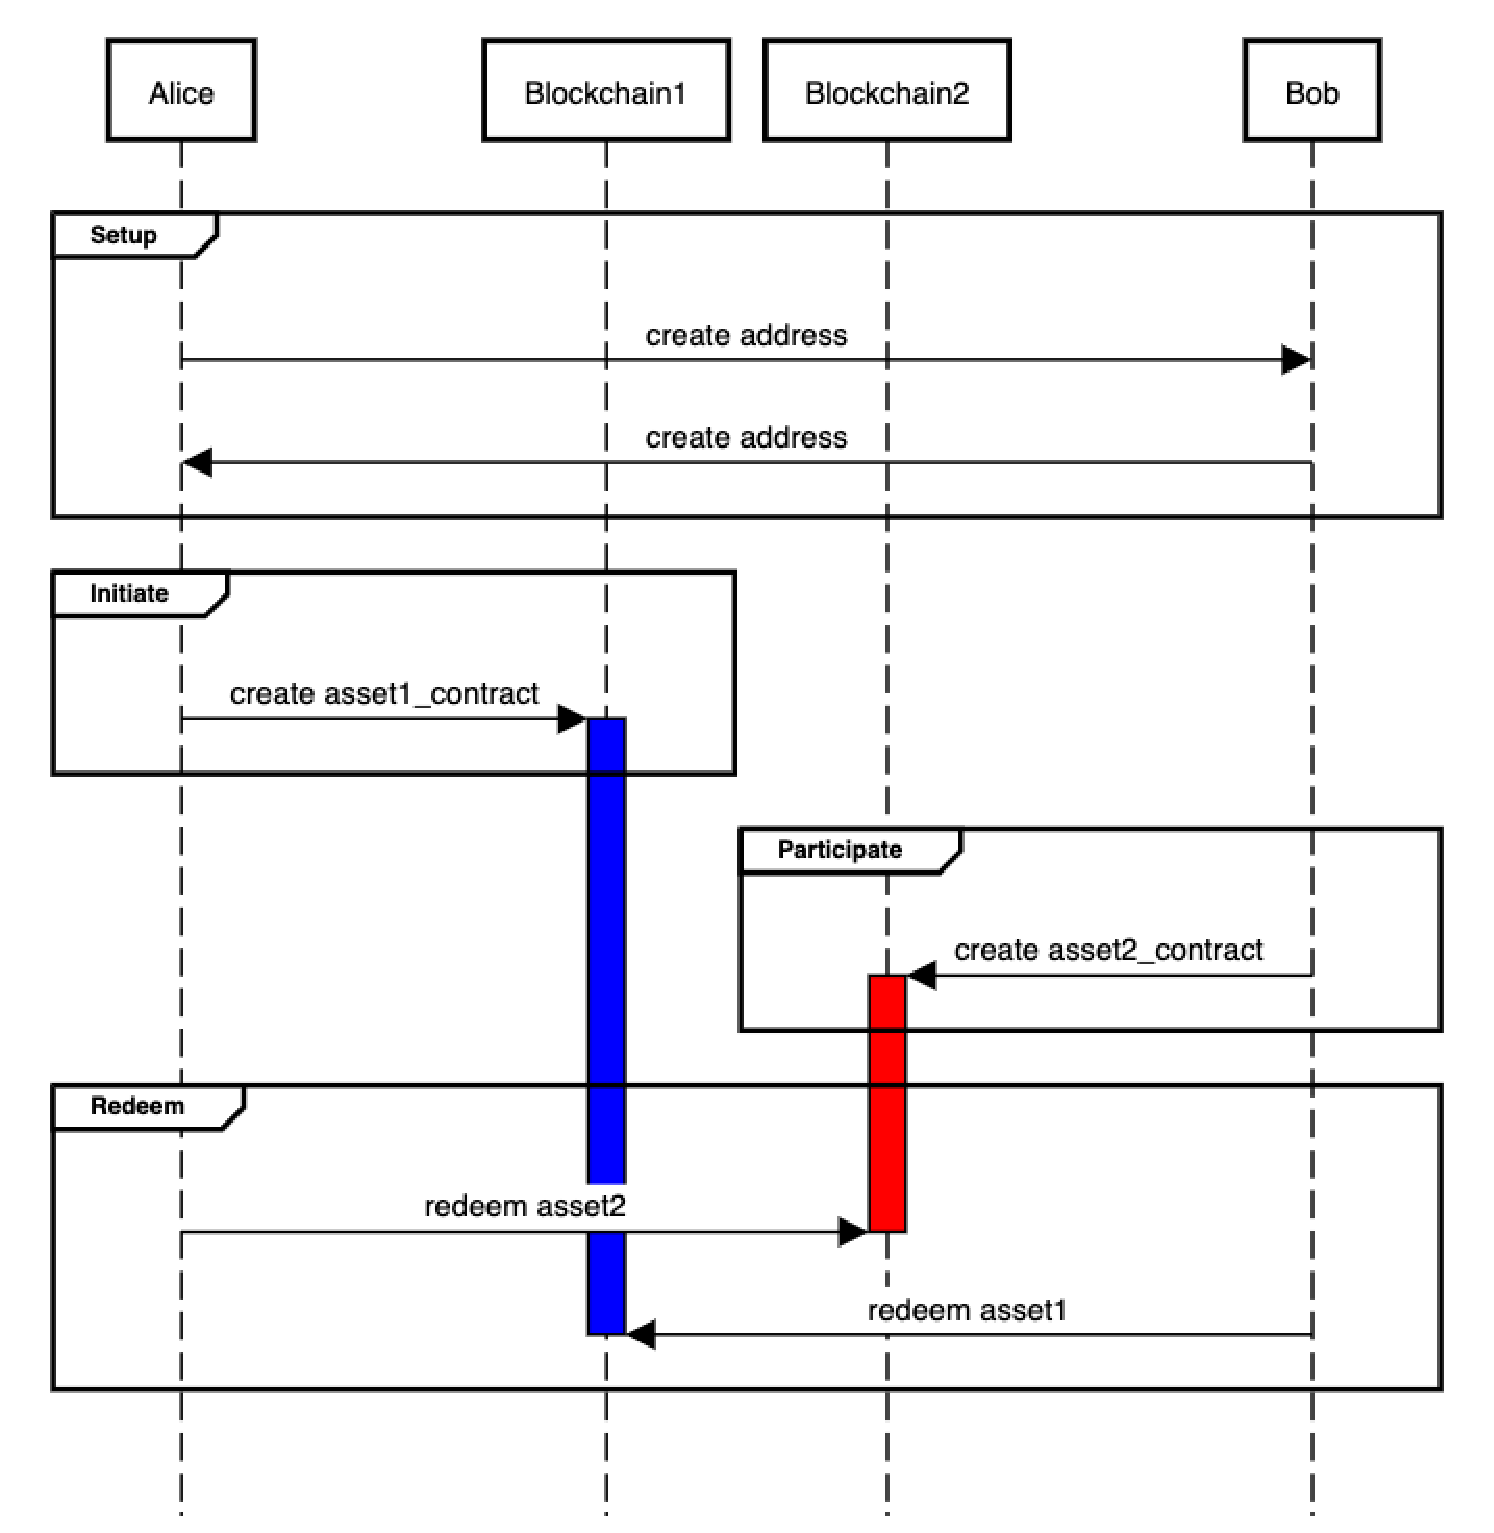
\includegraphics[width=\textwidth]{sequence_diagram_original.eps}
        \caption{Sequence diagram of the original Atomic Swap.}
        \label{fig:sequence_diagram_original}
    \end{subfigure}
    \quad
    \begin{subfigure}{.3\textwidth}
        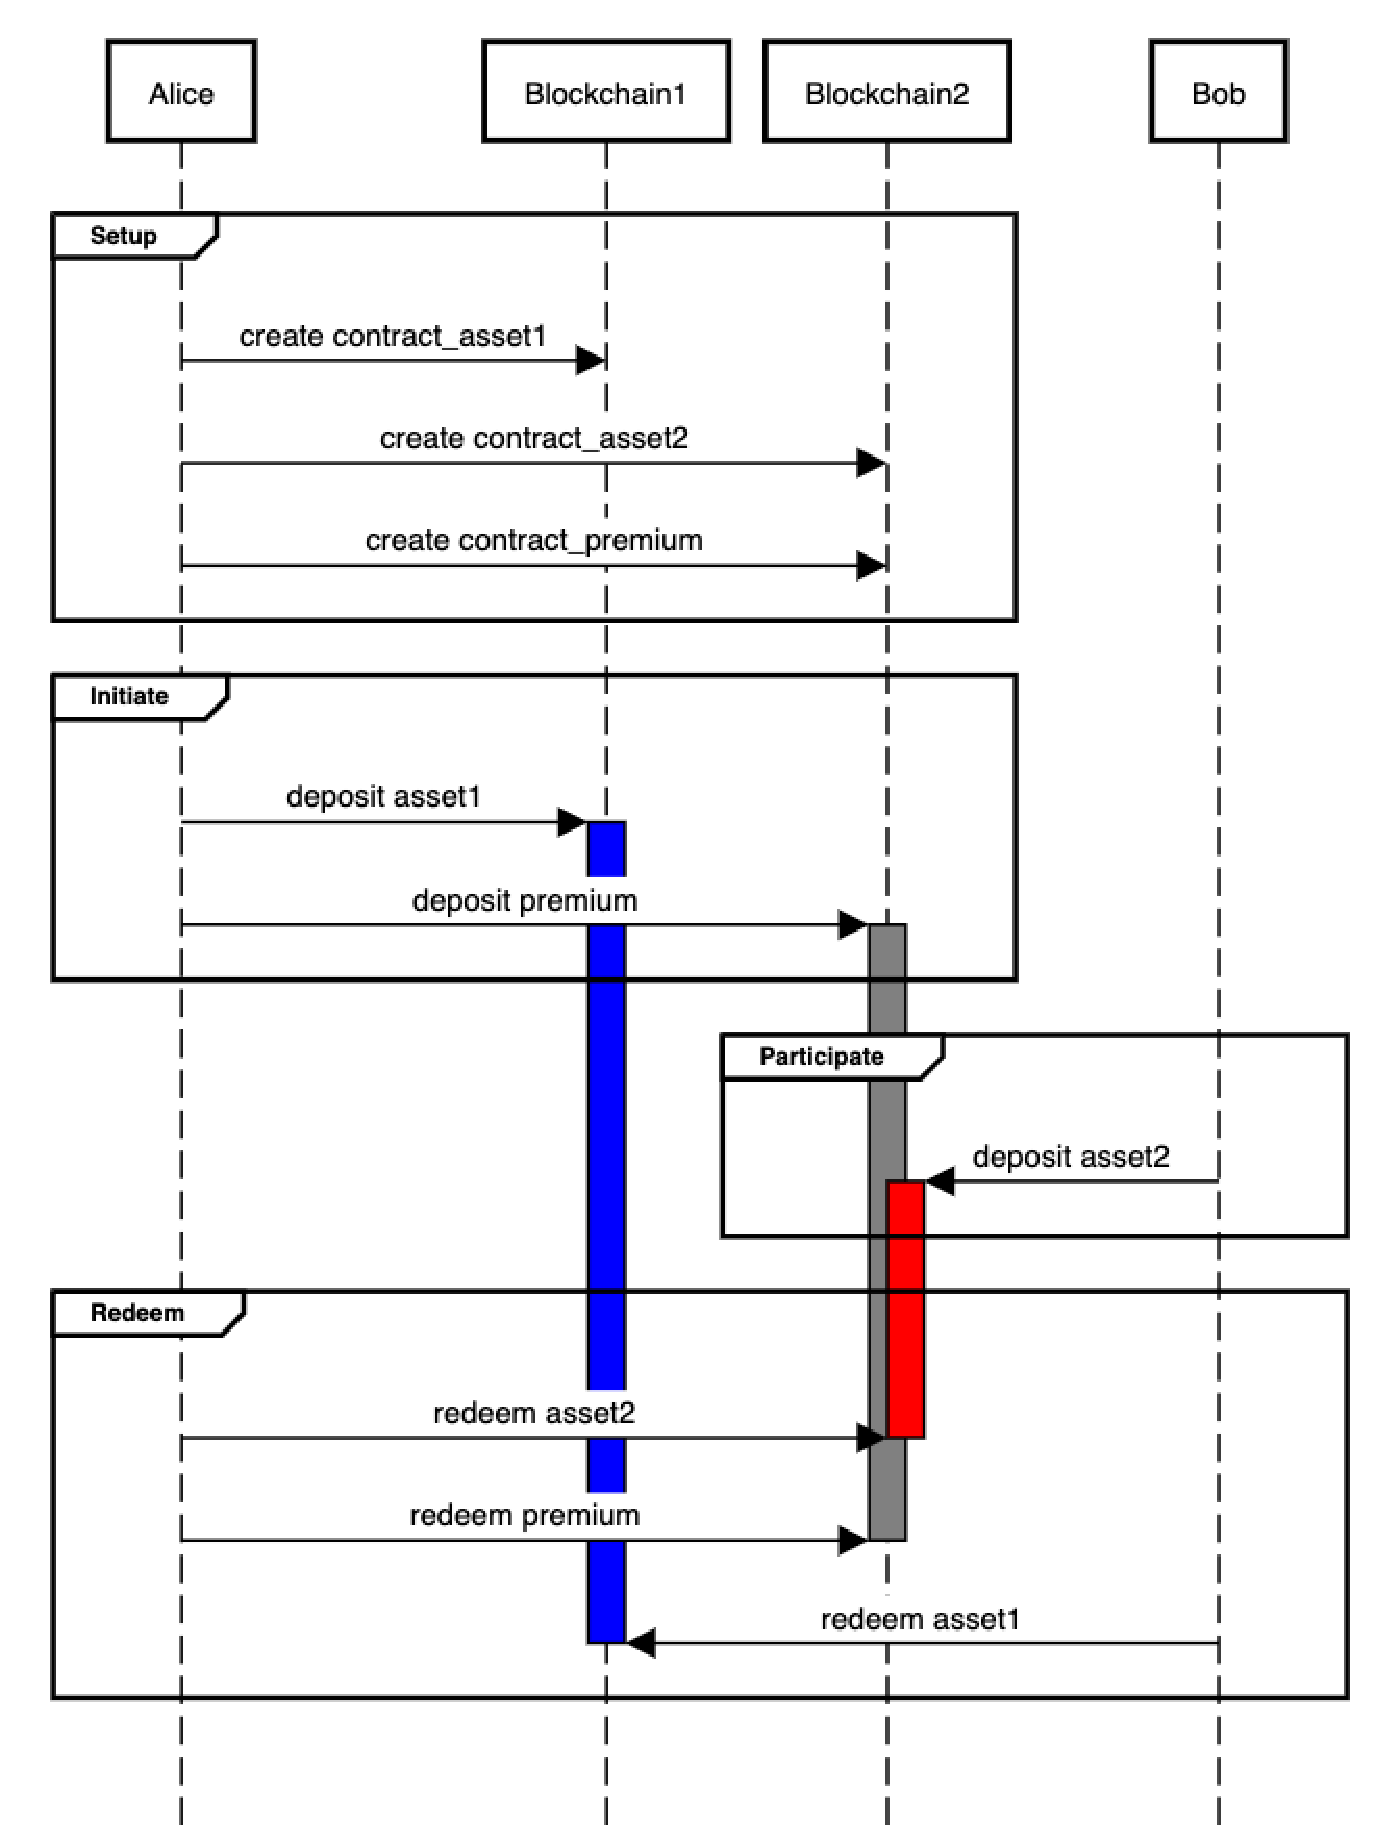
\includegraphics[width=\textwidth]{sequence_diagram_currency_exchange.eps}
        \caption{Sequence diagram of the currency exchange-style Atomic Swap.}
        \label{fig:sequence_diagram_currency_exchange}
    \end{subfigure}
    \quad
    \begin{subfigure}{.3\textwidth}
        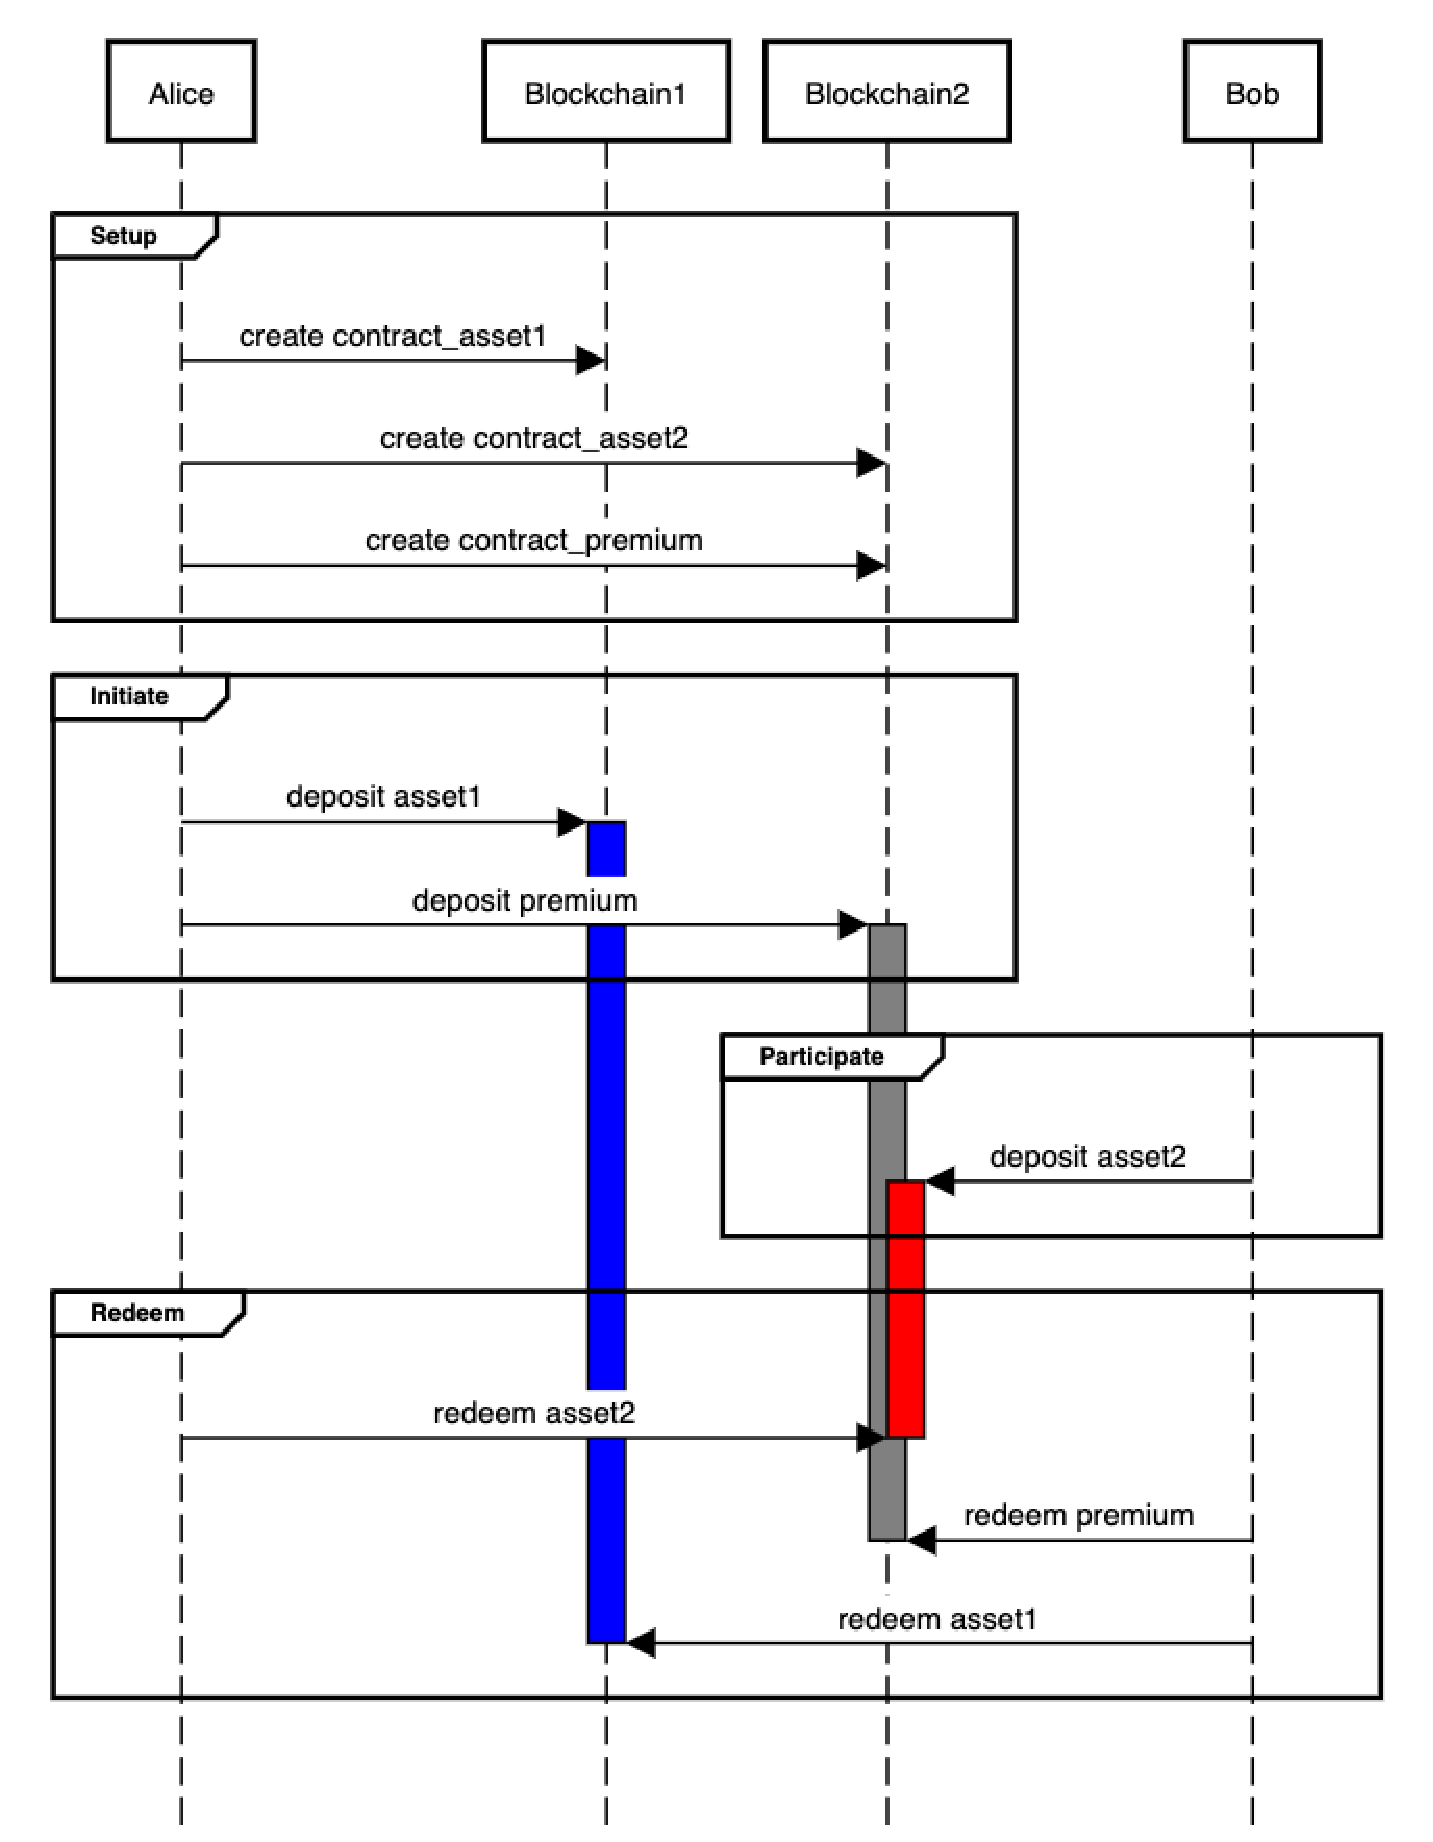
\includegraphics[width=\textwidth]{sequence_diagram_options.eps}
        \caption{Sequence diagram of the American Call Option-style Atomic Swap.}
        \label{fig:sequence_diagram_options}
    \end{subfigure}
\caption{Sequence diagrams.}
\label{fig:sequence_diagrams}
\end{figure*}

\end{document}
